\articlepart{Typin' Girls - はじめての競技タイピング}{W/H}

\begin{screen}
過去の記憶がお前に喜びを与えるときにのみ、過去について考えよ。\\
―― Jane Austen
\end{screen}

\section*{序章}

\begin{verbatim}
「いつから」と問われれば、あの日を境に。
僕は君を見ることをやめた。
君と僕のつながりはそうして強まって。
その不可視の糸は、切れることなく今もつながっている。

見やりもせず一心同体となる、一見理不尽な関係が。
日々思い慕いながらも、打ちつけるという関係が。
声こそ聞こえなくても、姿こそ見えなくても。
日々の交流を通して深まってゆくのを感じる。

僕らの交流は、極めて物理的なものだ。
けれど、その実それは極めて言語的でもある。

――物理と言語の界面<インターフェース>。

喩えるならば、それは果てしない大河だろう。
そこに、気が遠くなるような労力をかけ、橋をかける。
決して彼岸に届くことはないと知りつつ、橋をかける。
そんな戯れが、今の僕らの交流の形だ。

とするなら、あの出来事は、七の並ぶ日の夜空のような奇跡だったのだろう。
僕と君が、出会った日を思う。

ふわり、耳元を春風が吹き抜けていった。そんな気がした。

季節は冬。
暖を取らねば震えるような気温の中、懐かしさとかすかな喪失感をも振り払うかのように、洗面器の湯に浸していた両手をタオルで拭う。

ゆるみきっていた姿勢を正す。目がさえる。
ほかほかと熱を帯びた手をそっと、あるべき位置に。
人差し指の腹で、小さな突起をそっとなでる。

意識を、肩に、腕に、手首に、指に、
――鍵盤<キーボード>に。
そして真っ白な雪原に踏み出すように、軽やかに、親指を弾ませた。

カタン。
新雪降り積む窓の外、記憶の扉の鍵<キー>の音。
\end{verbatim}

\section{実力チェック}
\begin{screen}
競えば伸びる。\\
―― Typing Attack の合言葉
\end{screen}

\subsection{タイピング極めました(笑)}

始まりは僕が高校に入った春のこと。

どうしようもないほど位相がずれたインドア青春を送っていた僕だったが、ジュニアじゃないハイスクールに来てとうとう部活というリア充感漂うものに入らなくてはならなくなった。必須だったのだ。

しかし幸いかな、僕にはパソコン部という預言されしメシアがついていた。他の文化部に目もくれず(運動部という存在は、全く、存じ上げません!)メシアに入部届を出した僕は、初日の部活動で度肝を抜かれることになる。

……悪い意味で。

\answer{おじいちゃん先生}{新入生のみなさん。パソコンを使うには、えー、この、キーボード、と呼ばれる、文字の、色々書いてある機械と、マウス、という、ネズミのようなかたt(ry}

\answer{僕}{(レベル低っっっっっっ)}

\answer{おじいちゃん先生}{まずは、日本語を、パソコンに、入力……入力というのは、えー……キーボード、を使って、タイピングを、やるわけですが……入力! この練習から、始めたいと思います。}

\answer{僕}{(トロい! トロイア! トロイア戦争!(←三段活用))}

\answer{おじいちゃん先生}{ローマ字は、みなさん、ご存じですか?}

\answer{僕}{(Yes, I do! 実戦(← 2ch やニコ動への書き込み)で鍛えてる僕に隙はなかった!)}

\begin{screen}
こんなレベルの授業や部活動が実際に行われているところもあるそうで。
筆者の経験では、大学の英語の講義で 2 回に渡り A-Z タイピングをやるだけだったなんてことが実際にありました。英語やろうよ英語……。
\end{screen}

そう、僕は中学の時に自分専用のパソコンを買ってもらって以来、自室で多くの時間をテラワロスなどと打ち込みながら過ごしてきた。タイピングのイロハなんて釈迦に説法。なにしろ僕は、すでにタッチタイプ(キーボードを見ないで打つ超クールなスキルさ)ができないこともない、というハイレベルに到達しているのだよ。

実際、先生の説明することはすべて事前に知っていることばかりだ。IME のオンオフ、ホームポジション、母音と子音、シフトキー……。

退屈すぎて、おもむろにブラウザを立ち上げクオリティを発揮しようかという考えが支配的になってきた……その頃、ようやく面白そうな話になった。

\answer{おじいちゃん先生}{では、もうタイピングができそうだ、という人は、デスクトップにある、この、e-typing という、えー……ボタン、じゃない、アイコン、をダァブル・クリック(←年配の方がカタカナ語を発音するとき特有のテンション)してみて下さい。}

\answer{僕}{(e-typing ……いつだったかちょっとやったことがあったっけ? まあなんとでもなるよ)}

\begin{screen}
スコア帯別のアドバイスが次章にありますので、読者の皆さんでパソコンが手近にある方は、ぜひここで実際に e-typing の「腕試し」に挑戦してみて下さい。\\
\url{http://www.e-typing.ne.jp/}\\
会員登録しないでもトップページから「ランキングタイピング」→「腕試しレベルチェック」と辿ればプレイできます(2011/11 現在)。もちろん会員登録して、ログイン後にプレイしても構いません。
\end{screen}

\answer{僕}{(今週のテーマは「元気が出る言葉」らしい。どんな文章だろう)}

\answer{僕}{(元気出るどころか、なんか、え、つらいけど……? あれ……涙が……?)}

\answer{僕}{(いやいや、集中だ。ザ・アンダーグラウンド・ネットワーク(←2ch やニコ動)で鍛えた秘められし力を解放するときだ……圧倒的スコアを\ruby{叩}{たた}き出せッ)}

カタ……カタ……カタ……。

僕の指先が光の速さで\ruby{迸}{ほとばし}った。\ruby{疾}{はや}い……圧倒的じゃないか我が軍は。

伸ばし棒 \key{-} や位置が悪い \key{B} \key{Y} を打つ所ではさすがに手元を見てしまうが、それ以外はほとんどタッチタイプ。僕のタイピングはタッチ時々チラ見、いいね、いい速度だよ!

\answer{おじいちゃん先生}{ほう! 君はすごいね、映画にでてくる、あれだァ、ハッカァ! みたいだね。}

\answer{僕}{い、いえ……別に……(おおおおおおい気が散るよ! あとちょっとなんだ黙って!)}

ピピッピピピッ。

\answer{僕}{(桂ァ、今何ミス!?)}

……。オツカレサマデシタ。

\answer{僕}{(終わりか……微妙だなぁ、誰かさんの妨害のせいで……)}

「腕試しタイピング」が終わり、結果画面が表示される。

\begin{figure}
 \begin{center}
   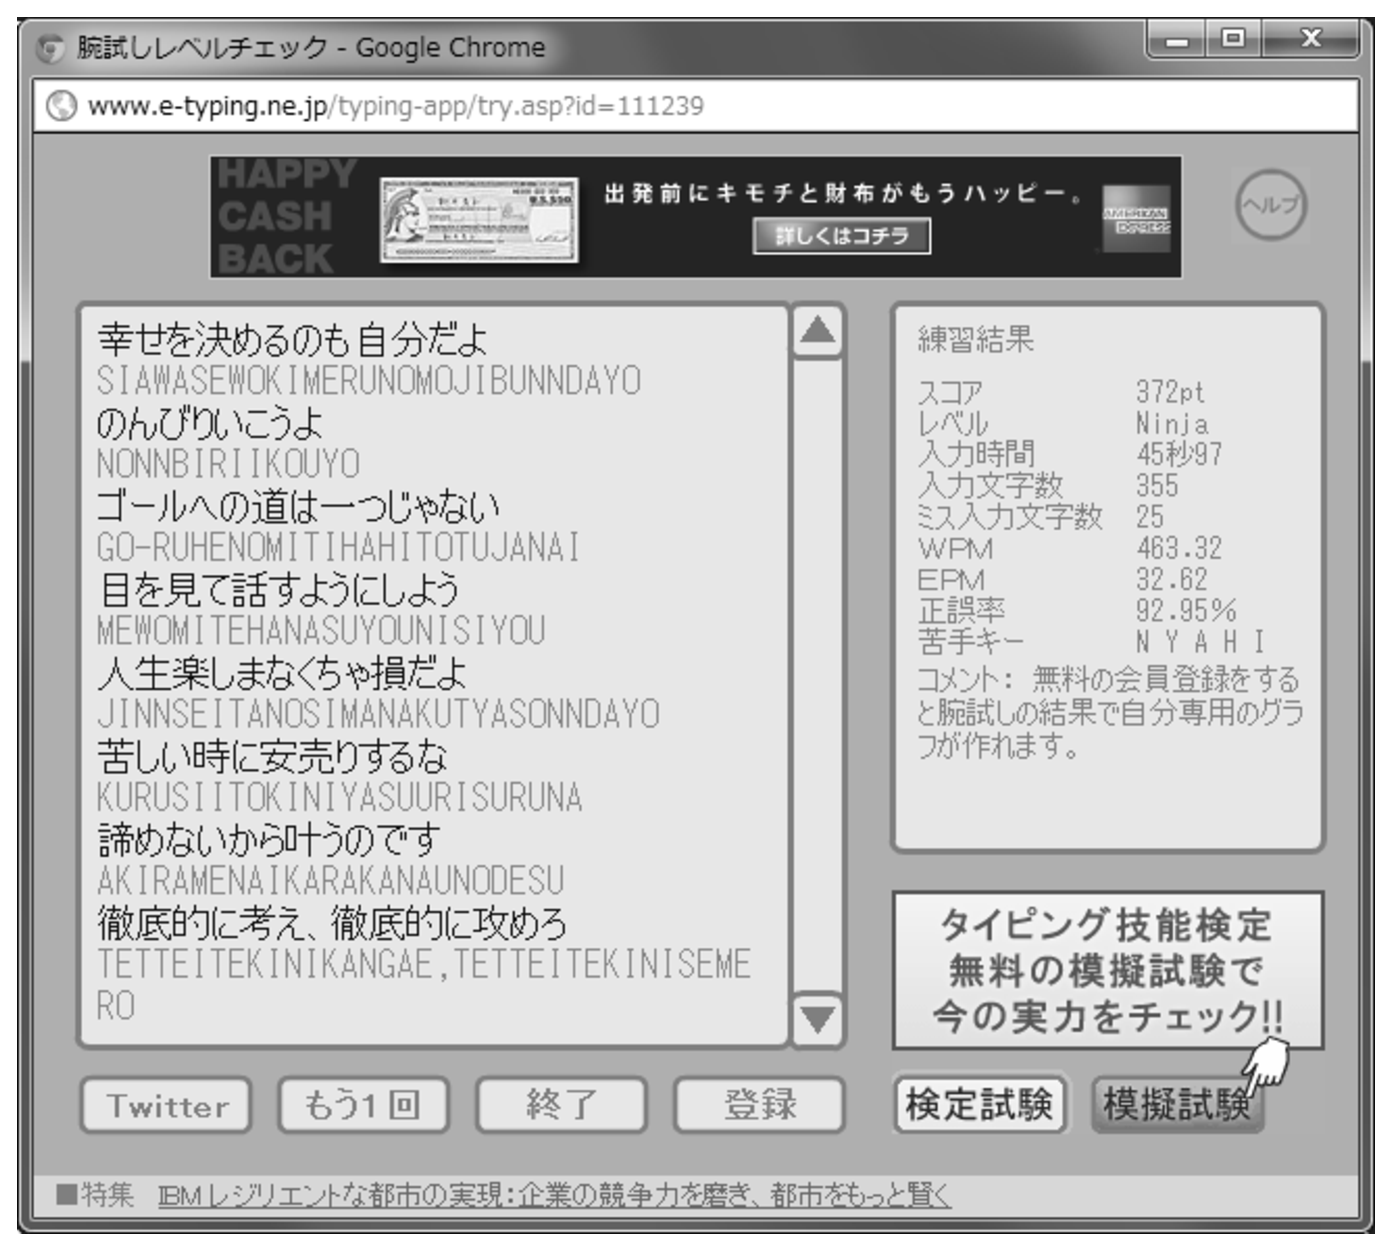
\includegraphics[width=7cm,clip]{res_x_i/ety_result1.eps}
 \end{center}
 \caption{e-typing結果画面}
 \label{x_i:ety_result1}
\end{figure}

\answer{おじいちゃん先生}{ニンジャ! ニンジャ、でましたよ! みなさん、372pt がでました。これはすごい、立派な記録ですよ。もっと速く打てた人、いませんか。}

\begin{figure*}
\begin{screen}
ここらで少々 e-typing について解説を。

最初に e-typing の紹介をしたのは、面倒な導入が不要で手軽にプレイして頂けて、かつ基礎的なタイピング力を見るのに適していると考えたためです。
e-typing の最大の魅力はユーザ数の多さで、ストーリーでもプレイしていた「腕試しタイピング」は毎週ランキングが更新されるのですが、各週のランキングに数千名が登録します。参加者数で見れば、間違いなく国内最大級のサービスです。
「腕試しタイピング」の他にも、入力する文章が様々に異なるモードがあります。「英語」や「長文」、「テンキー数字」など。
また同社が行っている「e-typing master」というタイピングの検定試験もあります。資格としての価値は正直なところあってないようなものですが、数少ないタイピング関連資格ではあるので、趣味でタイピングに取り組む際に目標のひとつにすると良いかもしれません(一番上の級「特級」は我々ガチ勢にとってもそれなりの難易度です)。

スコアについては、「僕」が 372pt で相当調子に乗ってますが、皆さんはどれくらい出るでしょうか。
ちなみに「僕」がプレイしていた「元気が出る言葉」という課題文のセットでは、全国ランキング登録平均スコアが 250pt 程度ですので、実際のところ「僕」のレベルはそれなりに平均以上ではあります。ざっくり偏差値で言うと 60 くらいでしょうか。

この記事は全体として、この時点における「僕」くらいの実力を持っている方を対象にして書かれています。つまり、タッチタイプが完全ではないにしろ\ruby{概}{おおむ}ねできて、実用上困らない程度には速く打つことができる人ですね。副題が「はじめてのタイピング」ではなく「はじめての競技タイピング」なのはそういうわけなのです。
したがって、タッチタイプがままならない方、とつとつとしか打つことができない方に対するフォローは残念ながら十分ではありません。このような同人誌に興味を持つ層であればまず問題ないラインと想定していますが、該当される方はごめんなさい。

なお、e-typing 攻略法については、まもなく登場するヒロインが、次章で解説してくれます。この章はほぼ伏線回収のための駄文だよ。やったね。
\end{screen}
\end{figure*}

だが周りの新入生はまだ黙々と、ピッピピッピと音を立てながら取り組んでいる。まだ打ち終わっていないのだ。

やや離れた所にいた、便乗して取り組んでいたらしき上級生の何名かも、見れば悔しそうな顔……。

つまり、僕の時代か。パックス・オレーノ、来ましたか。

\answer{僕}{ちょっと速すぎましたかね……。}

「ちょっとミスしすぎですかね」と言おうと思ったのに、つい本音が出てしまった。

だがしかし周りからは羨望の眼差し。冷静を装おうとするも、つい頬がつり上がってしまう。

\answer{おじいちゃん先生}{ニンジャ! 君のあだ名はニンジャね!}

\answer{僕}{(UZEEEEEEEEEEEEEEEE)}

こうして初回の部活動が終わった。成果は上々。

こんな感じでタイピングの神として君臨し、統治はせず、つかみはオッケーでゆるーく部活動を乗り切ることができるかと思うと、帰りの足取りは軽かった。というかスキップだった。

\subsection{タイピング界からの使者}

その日の夜、どこぞの運動部のように飯・風呂・寝るの確殺3連コンボを決めるわけがない僕は、帰宅後3秒で当然のように鞄から教科書を取り出し宿題と明日の予習を、やるわけもなく、パソコンの電源を入れ電脳空間へのダイヴ・フェイズへと移行した。

カスタムしてある愛機のログイン画面に、お手の物のタッチタイプでパスワードを\ruby{叩}{たた}き込む。パスワードのような、いつも同じ内容だと打つのがさらに速い。ダカダカダンとパワフルにマジカルにエクストリームに、

\answer{精}{いたたた! いたい、まだ用意できてないですし! ちょっと待っタンマ!}

どこからか声が聞こえた。

まあ、なに、珍しいことでもない。僕クラスになると想像力\ruby{逞}{たくま}しく幻聴が聞こえたりもするのだ。ラノベではないので驚いてやる義理もない。

スルーちからを発揮してダカダカダンとパワフルにマジカルにエクストリームに、

\answer{精}{痛いって言ってますよー無視しないでお願いあいたっ。}

今度は僕の目の前に――否、正確を期すれば、僕のキーボードの上に浮かび上がるように――確かに声の主らしきソレが現前した。

ソレというのはつまるところ、いやつまらなくても、このミニチュアロマン溢れる、ちんまいレディだ。年齢じゃなくてスケールがちんまい。何分の一フィギュアだ君は。

ちょうどキーボードのキーひとつの上に片足が乗るサイズの彼女は、どうも頭を打ったのか、セルフになでなでしながら表情を整えて、

\answer{精}{……ふぅ。気を取り直して、やっほー元気、はじめましてこんばんは。JST 的にこんばんは。}

どうしたことか、幻聴に続いて幻覚まで……などと認識否定を繰り返すのはまだるっこしく、僕もその手のフィクションでイラッ☆とする部分だ。

こんなこともあろうかと! 前々から万一自分の身に起こったらどうするかと、妄想もとい練ってきた策を発動する時がやってきた。僕はこの展開を自らの手で速攻、打破してみせる、速攻――即ちこうだ。

\answer{僕}{――君は霊か天使か女神か選ばれし現代人か異世界人か宇宙人か地底人か未来人か波動生命体か伝承存在か並行世界存在かメタ存在か妄想か脳腫瘍か視覚素子インプラントな拡張現実かオーパーツか人工知能高次元ホログラムか一体ナンデスカッ?}

はあはあと息が上がってしまったが、一気に言い切った満足感で(いやおそらくは酸欠のために)僕は言い知れぬ\ruby{恍惚}{こうこつ}感に包まれた。

そして気づく――死神とかダーク路線が手薄だ。

しかし、この光という光が泡立つ感覚の中魂どっきゅんと昇天するなら、それはありかナ――。

\answer{精}{タイピングの精です。かつタイパーです。typeする人でtyperと綴ります。英語的にはtypistが一般的とか言いっこなしで。}

なかなかやるな……平然と答えてきた。でも。

\answer{僕}{いや待った。自由解答じゃ困ります。上記の選択肢から選びなさい、複数選択可。}

\answer{精}{メタ存在と女神と未来人と並行世界存在と人工知能拡張現実と脳腫瘍がかすっていてあわせて 4 割、残り妄想という感じ? です。}

6割妄想かぁ! やっぱりね! 妄想に妄想ですと自己主張されるあたり、なるほど妄想じみている。

\answer{僕}{妄想メイン……じゃ害はないと? 危害を加える可能性しかないならご退散頂きたいし、危害あるかもだけどオイシイイベントもあるなら詳細聞くし、今すぐオイシイなら頂きますし、特に危なくもオイシクもないなら、自分の存在・文脈・世界設定について語れるだけ語っていって欲しい。僕がどうするかは、その後で決めよう。}

\answer{精}{適応力高すぎで私何も言うことないんですけど……その中では最後になりますか。オイシクなくてごめんなさい。オイシイのは厚くて熱いタイピング同人誌じゃなくて、薄いトリプルエックスなそれを別途お買い求め下さい。\footnote{この元ネタは gummi さんのツイートを参考にしました。勝手に加工・利用してすみません、感謝!}}

\answer{僕}{お買い求め? まあ、そのボディサイズじゃ色々あれだよね……(いや妄想メインならなんとでもなるんじゃ……いやまあ、設定を把握してからにしよう……)オーケー語って。}

\answer{精}{いいんです? ちょっと長くなるかもですよ?}

神妙な顔を作ってうなずく。僕の心が動かされれば、協力を惜しむつもりはない。

こういう不思議存在がコンタクトを取ってくる場合は決まって、何か困っているからだし。

\answer{精}{繰り返しになりますけど私、タイピングのアレです。ことタイピングに関してはエキスパートなタイパーのアレです。なんだっけ……精です、精。私に関して言えば、どこにでもいます。遍在してます。霊的なのです。えへん。で、今はキーボードの上に見えてますよね。半透明ですよね。これは\ruby{憑依}{ひょうい}的なアレで、この物理媒体と計算資源を通してあなたの認識に間接アクセスしています。ハイテクバイオです。えへん。この状態だとキーボードと一体化してるんで……こっちが準備してないのにダカダカと打たれると痛かったり。事実痛かったです。あ、もう大丈夫ですけど。それで、あなたと意思伝達ができてますけど……これは私の力だけじゃなくて、あなたと波長位相的なアレが合わないと無理です。だからあなたは選ばれし(というと聞こえは良いが要は妄想癖の)人的なアレで、ラッキーです。えへん、じゃないか、ぱちぱち。私の核というか本質はもっと抽象的で高次なアレですが、あなたの認識を必要とするという意味では属人的です。……これくらいで、私についてはわかります?}

\answer{僕}{組み合わせはわかった(←見栄)けど……その詳細が知りたいんじゃん。オーバーテクノロジーと証明可能な神秘学を手中に収め現代科学をあざ笑いたい。}

\answer{精}{はい無茶振り頂きました! っていうかそれやったらページ食い過ぎですから! 掘り下げたいのそこじゃないですから! ストーリーめちゃくちゃですから! ……はい、メタです。えへん。で、ですね……掘り下げたいのは「タイパー」の方なんですよう、私はタイパーの精なんですよう、「タイパーって何?」って聞いて下さいよう。}

\answer{僕}{(うわ……口が勝手に……)タイパーって何?}

\answer{精}{厳密な定義はない(諸派あって面倒です……)けど、ここではこう言っちゃいます。「タイピングを入力の手段としてではなくて、目的として行っている人たち」です。これくらい打てれば実用上十分……とかケチなことを言わないで、タイピングそのものを楽しみだしちゃったと。もっと適当に、「タイピングに情熱傾けちゃってる人たち」でも遠からずですね。そのタイパーの代表として私は来ました。すごい無理矢理がんばって、山ほど設定引っさげて、あなたの元へエッチラオッチラ(←こう書くとややエロい)やって来ましたんですよ。なので、言いたいこと言っちゃいます!}

ここまで聞いても、僕は彼女が言わんとすることが読めていなかった。

彼女が僕のタイピングに惚れ込んで、タイピングが世界を救うんだ宇宙で\ruby{隕石}{いんせき}を高速タイピングで打ち落とす人が必要なんだーとかいう話が出てきて、僕がヒーローになるというお花畑を幻視しているのみだった。

――だから割とショックだった。

\answer{精}{ええとですね、まずあなたは調子に乗りすぎなのです。の・り・す・ぎ・な・の・で・す! 井の中の\ruby{蛙}{かわず}です。凡百です。普通です。いや別に普通なのはいいです。でもそれで僕すげーって満足されちゃうと、私がむずむずします。黙ってられないです。世界を見せてやりたくなります。It's a typer world. ブルってる? と言いたいです!}

……何が何だか……わからない……。

タイピングなんかで凄まれる日が来ようとは。それも、こんなデフォルメチックミニチュアガールに。つついちゃうぞ?

\answer{僕}{つ、つまり、タイピングの精として、僕をパニッシュしに来た!?}

\answer{精}{別に罰しないですョ? タイパー優しいです。変人ではあっても愉快な人たちです。あなたはタイピングの基礎力もあって、人と競うことに価値も感じるタイプみたいなので、お仲間になれるんじゃないかなと思って。}

先ほどの凄んだ表情から、一転にこり。

つまりそれは勧誘だった。壮大な展開も、泣ける設定もなかった。

無論のこと、心など動かない。動きようもない。

……そんな風に思っていた時期が、僕にもありました。

\subsection{タイピング始めました}

想像できるだろうか。夕食を終えるなり両親との会話もそこそこに部屋に籠もり、(本人\ruby{曰}{いわ}く)半分オーバー妄想らしい存在と盛り上がる、(主に頭が)かわいそうな年頃の学生の姿を――僕である。

\answer{精}{お腹もふくれましたところで、現実を直視して頂きたいと思います。}

\answer{僕}{いや今というまさに今、妄想を、非現実を直視してるけど……。}

\answer{精}{\ruby{刮目}{かつもく}せよ! これが全・日・本レベル! 私の還る大・海・原! です! じゃん!}

\begin{figure}
 \begin{center}
   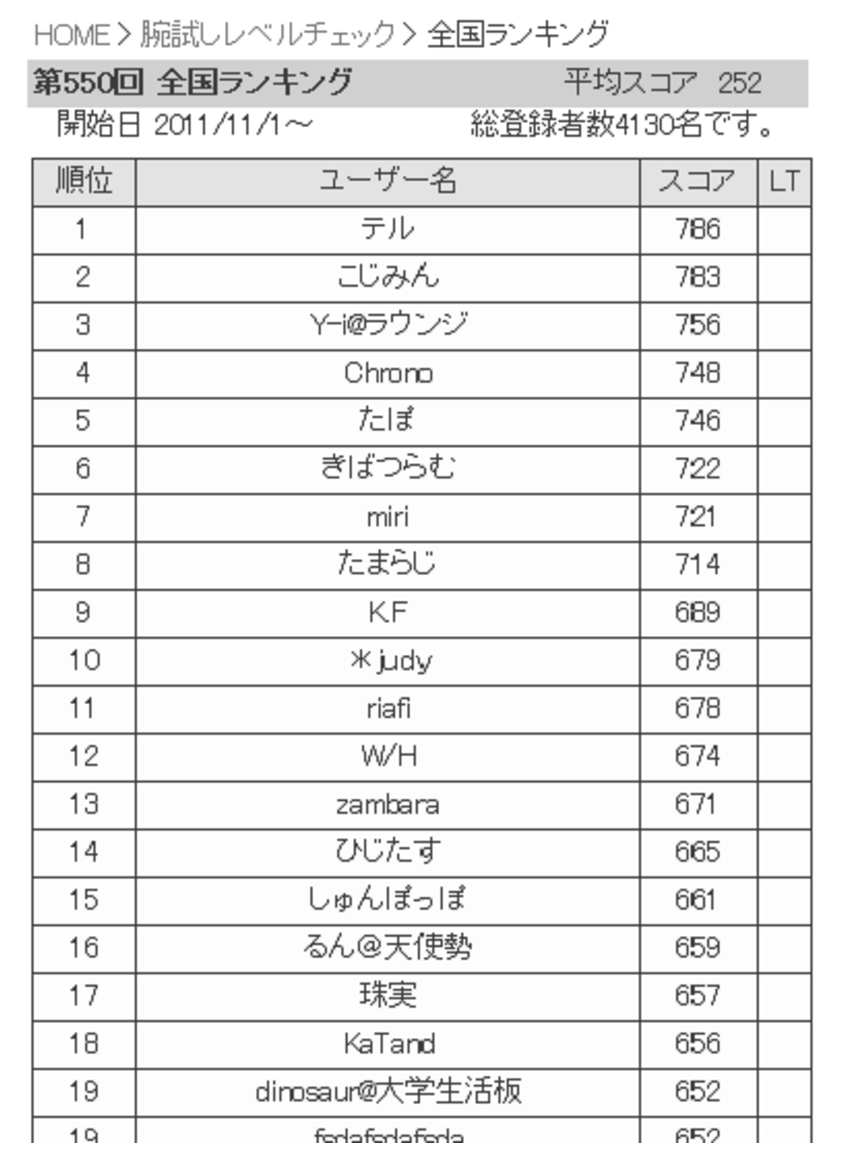
\includegraphics[width=7cm,clip]{res_x_i/ety.eps}
 \end{center}
 \caption{e-typing腕試し全国ランキング}
 \label{x_i:ety}
\end{figure}

\answer{僕}{えええええ!!(←約一名の自室に響き渡る近所迷惑な声)}

……ってなんすかこれ。一瞬でリアクションできる凄さ、どこにもないっていう……。テンション合わせてあげた僕、アホの子みたいっていう……。

\answer{精}{全・日・っp}

\answer{僕}{いやもうそのテンションいいんで、解説を。}

\answer{精}{はい。(←真顔)これは、学校であなたが打って 372pt を\ruby{叩}{たた}き出していた e-typing 腕試しモードのスコアの全国ランキングです。週ごとにリセットされるので、歴代のランキングとかじゃなくて、その週に出された記録しか入ってないですけど。}

\answer{僕}{わーすごい(←真顔)。チート使いばっかで荒れてる。}

\answer{精}{え、チート違いますよ?(←真顔)ガチですガチ。ガチタイパー勢です。}

\answer{僕}{いやだって……え?(←変顔) ウソでしょ? トップで 500pt とかだろ常識的に考えて……。}

一位のやつ、僕の倍以上スコアあるって?

大体、700 超えは若干名しかいないのに、600 後半はたくさんいるってのは……。

あれ? ってことは 600 後半の団子はガチってことに……いやいや 600 って…… 600!?

\answer{僕}{一位はチートじゃ? 「テル」って「チート」の変形もじりで自主申告してるし。}

\answer{精}{断じてチートじゃないですよう。現代の生きる伝説テル・ぶったーさんになんてことを……。}

\answer{僕}{え、でも……うーん……まあ、600 くらい出せる人がいるのはわかった。700 とかは眉唾かな。}

\answer{精}{(歴代トップだと 800 オーバーですけど……)いいでしょう、600。}

\answer{僕}{それくらいだったら、僕もやれば出せそうだけど。}

\answer{精}{今のままじゃ無理無理、絶対無理。っていうか、600 って私もそれくらいですし。}

\answer{僕}{え? そういえば君もタイパーって言ってたっけ。……出せるの? ってそのボディサイズじゃ無理じゃね?}

\answer{精}{見たいです?(←見せたくてうずうずしてる) 方法があるんですよー、これが。じゃあちょっと、お手をこちらへ。}

言うなり、キーボードの上からこっちこっちと手招く「精」(こいつ結局名前なんなんだ)。

先に説明すればいいものを、にこにこしたまま、黙って彼女は僕の手に触れシュイィーン! シュイィーンって!? シュイィーンって!!!

僕の肩から先の感覚はすぅっと、ろうそくの火でも吹いて消すかのように消えてなくなった。

\answer{僕}{ヴぁうおぁあああああああ腕がぁああああ! 僕の腕がぁああああああああああ!}

\answer{精}{あ、ごめんなさい。うずうずしちゃって説明が遅れました(てへっ)。こうやって\ruby{憑依}{ひょうい}すれば物理的に打てるなぁと……。}

見れば、確かに、腕は、ついている。

取れていない。痛みはない。

\answer{僕}{あああ……はうわっ、うおゎ、ぅわーお……(←目がマジ)。}

\answer{精}{一時的に借りてるだけですよ。ちゃんと戻せるし戻すので、そんなに焦らなくてだいじょぶです。目がマジにならなくてだいじょぶです。セーフです。}

\answer{僕}{お、オーケィ……。}

とは言ったものの、額には冷や汗が残る。いや、だってこれ、\ruby{憑依}{ひょうい}って……この感覚、普通じゃないよ。アブノーマルよ。妄想 6 割とか言ってたから油断しきってたっての……彼女の気分次第じゃ実害ありまくりじゃない。

だが当の彼女はというと、

\answer{精}{非ログイン状態でいっかー、おっけー、元気ワードね。実は長いだけで打ちやすさそんなでもないけど……ワード末尾の「できる」とかカモってるし、ま 600 は何度かやれば……!}

ノリノリである。本当にうずうずしていたらしく、僕はアウトオブ眼中。

\answer{精}{じゃ打ちまーす。}

感覚がない僕の腕から下が、僕の意識を通さず勝手にキーボードを操作していく。僕の手でありながら僕の手ではないという奇妙な体験。

この\ruby{憑依}{ひょうい}現象に文字通り全身全霊でびびって震え上がった僕は、彼女の気分を損ねないように、適当にスゲーとかヤベーとか言おうとヒヨっていて。

そして――言葉を失った。

ッタカタタタタタタタタタタタタタン!
ッタカタタ(ピッ)タタタタタタタタタタタタタタタタタタタン!
ッタカタタタタタタタタタタタタタタタタン!
ッタカタタタタタタタタタタタタタタタタタタタタタタタタタタン!
ッタカタタタタタタタタタタタタタタタタタタン!

音は弾倉交換しつつ撃ち続ける Machine gun なら、

手もコンピュータと同期し動き続ける Machine だった。

僕の手が勝手に動くという、恐怖感。僕の妄想でチートだろうという、非現実感。僕も何度かやればこれくらい出せるという、お花畑。それらがマシンガン音と残像の見えそうな指の高速移動に、撃ち抜かれ圧倒され吹き飛ばされる。

打ち終わって、一息ついたらしき彼女にかけるべき、いくつかの言葉が浮かんだ。

「ゴッデス! 君のあだ名はゴッデスね!」

「ちょっと速すぎますね……」

「Is it a typer world? 狂ってる……」

だけど、実際に口をついて出てきたのはこれだ。

\answer{僕}{タイピング、始めたいです。}

\begin{screen}
主人公と同じ気持ちになりたい方は、動画サイトにある高速タイパーのプレイ動画を見ましょう。
以下にいくつかおすすめのものを載せておきます。どれも魂が抜けるレベルです。

\begin{itemize}
 \item (ニコ動) sm8243869 あきうめ氏の「慣用句」798pt
 \item (ニコ動) sm13155297 あきうめ氏の手元
 \item \url{http://youtu.be/4YzFkzRbOcg} ひろりんご氏の「思い出の言葉」810pt
\end{itemize}
\end{screen}

\section{e-typingで基礎力を}
\begin{screen}
ミスをするくらいなら打つな!\\
―― 正確性重視を強調する、全日本タイピスト連合のキャッチフレーズ
\end{screen}

\subsection{敵を知り己を知らば}

無事に腕の制御を取り戻した僕は、早速彼女の話に耳を傾けていた。

\answer{精}{まずは姿勢です、そのやる気ない感じのそれをなんとかして欲しいです。}

\answer{僕}{なるほど把握、姿勢が重要なのは何やるにしても基本だね(シャキッ)。}

\answer{精}{いや現段階だと姿勢とか誤差です。}

\answer{僕}{と、言うと?}

\answer{精}{座学やるので、まじめに聞いて欲しかっただけです。}

\answer{僕}{あ、はい。}

\answer{精}{敵を知り己を知れば百戦危うからず! ……と偉い人は言いました。ということで、自分ってどれくらいの腕前だと思います?}

\answer{僕}{ふむ……けっこうすごいと思ってたんだけど。}

\answer{精}{そうです、けっこうすごいです、実際。}

\answer{僕}{こき下ろしたり持ち上げたり、どっちなん打!(あれ、なんだこのカンジ……)}

\answer{精}{一般人的には「すごい」んです。だって普段文字を入力するときに困ることなんてないでしょ? これなら。}

\answer{僕}{そういう意味じゃそうかな? ネトゲでチャットするのも、ブログ書くのも楽勝だしねぇ。}

\answer{精}{そう、普通にパソコンを使う時の入力手段としてなら、十分です。}

\answer{僕}{でも……さっきのあれ見ると、まだまだかなって。}

\answer{精}{ここから先は、言ってしまえば、基本的に遊びの領域です。文字の入力をお仕事にでもしない限り、見返りはあまりありません。だから「競技タイピング」と言っています。}

\answer{僕}{技を競うって書いて「競技」か……。}

\answer{精}{100m を 13 秒で走れる人が、がんばって 10 秒で走れるようになっても、そんなの日常生活ではほぼ何の役にも立たないですよね。でも陸上選手から見たら、その差はものすごいですし、10 秒で走れる人には賞賛が送られます。スポンサーもつくかもしれません。つまり陸上という世界の中では「10 秒で走れる」という、そのこと自体に価値があるわけです。私たちのいる競技タイピングの世界も、陸上と比べちゃうと小規模ではありますけど、そういう場所です。だからさっきは「井の中の\ruby{蛙}{かわず}」なんて言い方をしましたけど、井の中は井の中で快適です。困らないし、悪くないです。引き返すなら今のうち……ですよ?}

\answer{僕}{井戸ごと海に放り込んだのは誰ですかね……でも、いいよ。とりあえず君の記録はすぐ超えてみせるから。}

\answer{精}{わー、その意気やよし! やはり私の目に狂いはないですね。}

「役に立たない」と断言されて興味を失う人もいるんだろう。

でも、それを言ったら、僕の普段プレイするゲームだってそうだ。音ゲーがうまくても、FPS がうまくても、基本的に役に立たない。でも、楽しいからやる。

楽しいと思えるうちはやってみよう――それが僕の出した回答だった。

\answer{精}{では、仕切り直して、次は敵を知ります。解説のため、あなたが調子に乗りまくっていたニンジャ記録の重要部分をぺたっと。}

\begin{figure}
 \begin{center}
   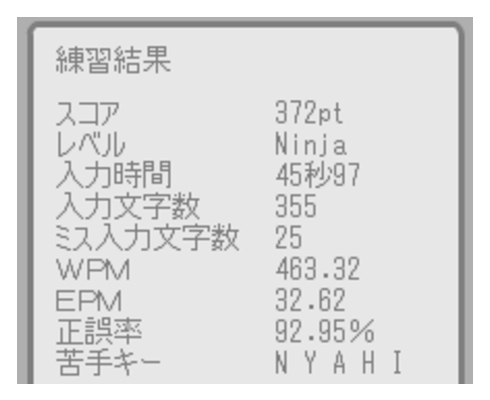
\includegraphics[width=7cm,clip]{res_x_i/ety_result2.eps}
 \end{center}
 \caption{結果画面の重要部分}
 \label{x_i:ety_result2}
\end{figure}

\answer{僕}{あれ、結果画面左の部分は見なくていいの?}

\answer{精}{左にはワードが並んでいるだけですからね、今は注目しないでいいでしょう。}

\answer{僕}{ワード?}

\answer{精}{タイピングゲームでの出題文のことです。英単語の word の意味通りに「単語」とは限りません。例えば、この e-typing なら、画面にひとつずつ文章が表示されますよね。この文ひとつひとつが{\bf ワード}と呼ばれます。まあ、ちゃんとした定義はなくて曖昧な感じですけど。ノリです、ノリ。}

\answer{僕}{なんとなく把握した。}

\answer{精}{ちなみに e-typing ではランダムに 15 ワードが出題されます。意味、わかりますよね。}

\answer{僕}{何か文章が表示されて、打って……と 15 回やったら終わりになる、と。}

\answer{精}{です。では各項目を解説しましょう。それぞれこういう意味です。}

\begin{itemize}
 \item スコア:結果から計算されたスコア。これで競う
 \item レベル:スコア帯に応じた称号
 \item WPM:一分間に何回正しいキーを打つスピードか
 \item EPM:一分間に何回ミスをするペースか
 \item 入力時間:入力を受け付ける状態だった総時間
 \item ミス入力文字数:ミス(誤打鍵)をした回数
 \item 入力文字数:正しく打った文字の数
 \item 正誤率:1 - ミス入力文字数 / 入力文字数
 \item 苦手キー:ミスが多かった部分のキー
\end{itemize}

\answer{精}{まず WPM が一番注目したくなりますね。}

\answer{僕}{タイピングの速度か。僕は一分間に 463 回、ってことは 60 で割れば……一秒間に 8 回弱。やっぱかなり速いよね。}

\answer{精}{ですね。最初は秒速に直して考えた方が大体のスピードがわかりやすいはず。でも、タイパーの人達は分速の方に慣れてます。その方が整数で表現できたり、大きい数になるので差がわかりやすかったり、メリットがあるので。まあ心配しなくても、多くのソフトでこちらが使われているので、そのうち分速の方に勝手に慣れますよ。}

\answer{僕}{EPMはWPMのミスタイプバージョンか。}

\answer{精}{正直なところ、あまり注目することはないですね。というのも「ミス入力文字数」も表示されるので、普通はこっちに注目します。}

\answer{僕}{これは単にミス回数だよね。}

\answer{精}{そうですけど、「何カ所でミスをしたか」ではないことに注意です。同じ部分で何回も間違ったキーを押すと、一回ずつこの「ミス入力文字数」にカウントされちゃいます。}

\answer{僕}{何回「ピッ」ってなったかってことね。「入力文字数」は……正しく打った文字の数ってことは、出題されたワードによって決まってくる数。}

\answer{精}{ほぼその考えで合ってますけど、実はちょっと違います。が、これはディープな話なので後回しで……「入力時間」「正誤率」についても、なんとなくで大丈夫です。}

\answer{僕}{「苦手キー」は間違って押したキー?}

\answer{精}{ではなくて、ミスをした箇所で押さなきゃいけなかったキーです。あなたの記録の場合\key{N},\key{Y},\key{A},\key{H},\key{I}を押さなきゃいけない場所でミスが多かったというわけ。}

\answer{僕}{レベルはスコアで決まるんだよね。最高のレベルまではやりたいところ。}

\answer{精}{その発想は……フフフ、危ないかと?(暗黒微笑)そしてお待ちかねのスコア計算式ですが、こうなってます、ででん。}

\begin{screen}
スコア = (WPM - EPM) $\times$ 正誤率の二乗
\end{screen}

\answer{僕}{へぇ。WPM - EPM が 430.7 だから、これに 0.9295 を二回かけて……372.111986675。確かにスコアの 372pt に合うね。}

\answer{精}{ここからわかることはなんでしょう?}

\answer{僕}{うーん……スピードが速いとスコアが高くなる。}

\answer{精}{当たり前すぎますけどね。……むしろ、速度である WPM をベースに、そこからしょっ引かれていくという見方が重要かな。もし引かれなければ、WPM がそのままスコアになるわけです。}

\answer{僕}{EPM が 0 で正誤率が 100\% なら、WPM がそのままスコアか。それってつまり……一回もミスをしないってこと。}

\answer{精}{Exactly(その通りでございます)。EPM も正誤率も、ミスに関係した数ですからね。ミスをすると EPM が増えて正誤率も下がる。しかも正誤率は二乗で計算されちゃうので……イメージとしてはミスのペナルティが三重につく感じです。三重苦です。}

\answer{僕}{この記録 25 回もミスってるじゃん(主に誰かのせいで……)、もしこれがなかったら、WPM がそのままがスコアで、463pt!}

\answer{精}{ミスが多すぎます。はじめからやり直してください。ミスをしないということは、ミスをしたことに気づいて打ち直す……っていうタイムロスもなくなるということです。だから今のあなたの場合、実はノーミスなら WPM も上がる余地があるってこと。}

\answer{僕}{500pt 完全に見えたよ、これ。}

\answer{精}{さあ、それはどうでしょーかね?}

キーボードの上に陣取る妄想生命体(なのか?)は、謎の笑み(=暗黒微笑)を浮かべるとそう言い残し、姿を消した。僕の目の前には、明け渡されたキーボード。

よし、やってやろうじゃないか。500pt の壁、速攻打破してみせる。ミスをしなければ大丈夫だ、問題ない。

\subsection{何戦してもまだ危うい}

それから数日が過ぎた。

あの日はどうも疲れていたようで、あれ以来、腕の感覚がなくなることも、おかしな幻覚・幻聴を体験することもなくなった……という展開になる可能性を 50\% 程度と想定していた僕だったが、現実は妄想に寛容だったらしい。今日も、部屋には打鍵音が響き渡っている。

\answer{僕}{……(ピッピッ)くそ……またミスって詰ま(ピッ)ってミス(ピッ)って詰まって……(ピピピッ)うううう!}

未だに 500pt を出すことはできていない。それどころか、450pt すらも出ていない。

\answer{精}{急ぎすぎなんですよ。}

\answer{僕}{でも、このスピードじゃないと……何度もやれば 500pt が出るはずなんだよ。奇跡が起きれば。}

\answer{精}{気持ちはわかりますけど、さすがに絶望的です。そろそろ気づいてるんじゃないですか? ある程度スピードを落とさないと、ノーミスなんて出ないって。}

\answer{僕}{ノーミスならスピードも伸びる余地があるって言ったの君だ! だまされた! うぼぁー!}

\answer{精}{言いました。言いましたが、今回すぐそれが達成できるとは言ってません……つまり、達成は 10 年後、20 年後ということも……。}

\answer{僕}{ひょおおおおおおおお!}

\answer{精}{という冗談はさておき。}

\answer{僕}{はい。(←ノリに慣れてきた)}

\answer{精}{エンジン全開で打って、運良くミスがなかったら……なんていう妄想的な打ち方をしていると e-typing は永遠に、アレです、クソゲーです。イライラ棒です。だからその逆、ミスを極力しないような打ち方で、どれだけスピードを出せるか、と考えるといいです。}

\answer{僕}{やってみるか……。}

\answer{精}{プレイ中に\key{Esc}キーを押すとプレイ中止、結果表示画面で\key{R}キーを押すとリトライできるので、活用してください。}

\answer{僕}{いや、それ最初に言ってよ……。}

―― 十数分後 ――

\answer{僕}{やっと出たし……ノーミス。}

\answer{精}{めでたいです。スコアは……。}

\answer{僕}{340pt。ダメじゃん! 最初の記録よりも下がってる! ゴミ過ぎる!}

\answer{精}{ミスをしないように打つのがいかに難しいか、わかったんじゃないですか。滅茶苦茶に乱打してノーミスなんて奇跡は、まずないんです。}

\answer{僕}{悔しい……けど感じちゃう……その通り。ミス数を抑えようとして打つと、すごく遅くなる。ビクビクして、速く打てないっていうか……。}

\answer{精}{(この歳にしてこのネタ根性……)でも、そこで無理して指を動かすと、ミスになっちゃいますよね。}

\answer{僕}{それそれ。でもじゃあ、速くてノーミスって……どうやるの?}

\answer{精}{魔法のような解決策はないです。でも、練習をすると、だんだんできるようになります。さっきも言った通り「ミスをしない範囲で速く」という意識でタイピングをすることは重要です。今はノーミス縛りでやってもらいましたが、必ずしもノーミスである必要はないですよ。はじめはミス 3 回までとか、それくらいを意識するだけでも十分、効果があります。}

\answer{僕}{そんなこと考えてタイピングをすることなんて、普通ないしね。}

\answer{精}{普段のタイピングシーンでは「適当に速く打ってミスしたら直す」か「速度は気にせず、丁寧にゆっくり打つ」かどっちかなんです。「速くて正確ぅ!」\footnote{元ネタは「バトル&ゲット! ポケモンタイピングDS」。}できれば最高なんですけど、なかなかそれは意識しませんよね。}

\answer{僕}{それを目指すなら、初心にかえって練習あるのみってことか。}

\answer{精}{そう。そしてそういう意味で「速くて正確ぅ!」なクールなタイピングの基本を身につけるには、e-typing のスコアルールは割と、ちょうどいいんです。ノーミスで打ってさえいれば伸びるというわけでなし、ミスを増やしてでも速く打てば伸びるというわけでなし。両立ができた時、良いスコアが出るようになっています。もちろん、運の要素もありますけどね。そこはゲームですから。}

\answer{僕}{意外と奥が深いから困る。}

\answer{精}{この程度で奥が深いなんて言っていたら……気絶しますよ?}

\answer{僕}{楽しみにしとく。}

と言ってしまってから、本当に楽しみにしている自分に気づく。

この時の僕は、わかったようでいて、何もわかっていなかったのだ。踏み込もうとしている世界が、一体どのような魔境であるのかすら。

\subsection{段階別攻略}

僕は正確性を重視して練習を重ね、とうとう 3 ミス 440pt という記録を出すに至った。ミスがなければ 450pt 超え。悔しさはあったが、もう 450pt は時間の問題だと確信できる。

そして同時に、500pt を改めて意識する――。

\answer{僕}{一番いい助言を頼む。}

\answer{精}{いろいろな要素がありますからね……段階によって大まかにアドバイスになりそうなことはありますが、個人差もありますし。読者さんのこともありますので、段階別に色々と見てみましょか。}

\subsubsection{~200pt}

\answer{僕}{じゃ、100pt とか 150pt とかの雑魚は?}

\answer{精}{言い方はどうかと思いますけど……でもごめんなさい、そういう方には練習してくださいとしか。パソコン入門的な本や初心者向けのタイピング練習サイトを参考にするのもいいですし、別に参考にしなくても、ひたすら打っても伸びる頃だと思います。e-typing にも「腕試し」の他に「基礎練習」「基本練習」のようなコンテンツがあるので、試してみるのもいいですね。}

\answer{僕}{キーの位置を覚えたり、ホームポジションからの動かし方を練習したりするやつね。}

\answer{精}{面白みがあまりないので軽視されがちですけど、伸ばし棒\key{-}や\key{P},\key{Z}みたいな小指の方にあるキーと、あと人差し指で幅広くカバーしなきゃいけない中央付近のキーは、後々まで苦手意識が残りやすい部分です。もっと速く打てている人でも、不安があったら良い機会だと思って練習しましょう。}

\answer{僕}{さすがに僕にそれは当てはまらないな。(←ハイフンのたびに減速してる人の台詞)}

\subsubsection{200pt~300pt}

\answer{僕}{250pt くらいが一般の人の平均らしいけど、このへんは?}

\answer{精}{そうですねぇ、例えば「き」なら右手中指で\key{K}\key{I}という風に打ちますよね。こういうひらがな単位での運動は、反復練習して無意識にできるようにすることが大事です。別にまだキーボードを見ていてもいいので、無意識に、ひらがな単位でまとめて。}

\answer{僕}{250pt もあれば、それはとっくにできるんじゃ?}

\answer{精}{かもです。個人差があるって言葉でお茶を濁します。ひらがな単位でまとめて打てるなら、今度は単語とかのレベルの「まとまり」を意識して練習するといいです。}

\begin{screen}
\begin{itemize}
\item[ ] みかんをたべる
\item[×] み/か/ん/を/た/べ/る
\item[○] みかん/を/たべる
\end{itemize}
\end{screen}

\answer{精}{このように認識しやすい単位に分けて、各部分はスムーズに打てるように。最初から「たべる」の 6 打鍵 TABERU をまとめては難しいかもしれません。その場合は TABE で 4 打鍵とか、もう少し細かく分けた所からスタートでもいいでしょう。ひらがな単位よりは長い部分を一気に、というのがポイントです。}

\answer{僕}{e-typing を始める前から気づいたらやってたな。}

\answer{精}{ある程度速く打てる人は、必ずこうやっています。できるようになると一気に速くなりますね。}

\answer{僕}{他には?}

\answer{精}{このスコア帯の人に限らないですが、ここから先は「もっと速く打とう」と意識して打たないと伸びていかないと思います。実用的な目的でタイピングをしている人などは、この程度のスピードでも特に不自由しないので、「タイピングとは、これくらいのスピードで考え、指を動かすもの」って速度の制限を無意識にかけてしまっていることがあります。もっと速くなりたいなら、ハングリー精神を持ちましょう。大丈夫、あなたの限界は全然こんなところじゃないです。}

\subsubsection{300pt~400pt}

\answer{僕}{300pt 以上ってなると……練習を始める前の僕くらいか。じゃ、この間言われたことの通りなのかな。}

\answer{精}{そうですね。タイピングに特化した練習はしたことがないけど、パソコンはバッチリ! 系の人はこの辺じゃないでしょうか? 繰り返しになりますが、焦りすぎず、正確性重視で打ってみることをオススメしたいレベルです。初めからノーミスなんていう人は少なくて、400 WPM 以上出ているけど、ミスのペナルティのために 350pt 程度、という人が多いですし。}

\answer{僕}{僕もそのタイプだったわけだ。あとこれさ、やっぱり慣れもあるよ。ワードの種類ってそんなに山ほどはないから、何度も何度もやってると打ち方がわかってくる。}

\answer{精}{週ごとにワードのお題、ワードセットが変わりますが、各セットは 100 から 500 種程度のワードからなってます。多いと思うかもですが、打っていればすぐ見たことのあるワードばかりになっちゃいます。ワードごとの癖が把握できていれば、もちろん打つのも速くなりますし、スピードを出せるワードはどれか、ミスしやすいワードはどれか、なんていう意識・調整もしやすいわけです。そうやって慣れることを{\bf ワード慣れ}と言っていて、もちろん重要ですね。}

\answer{僕}{それでけっこう伸びた感じがする。}

\answer{精}{ひとつ前で解説した、まとまりで認識、ということに関連して、{\bf 先読み}と呼ばれる技術もそろそろマスターしたい頃です。}

\answer{僕}{あーあ、イケてる名前の技が出てきちゃいましたね……僕の時には言わなかったくせに……。}

\answer{精}{いじわるじゃないですよ? あなたの場合は最初からできていたのです。名前は荘厳ですけど、実は大したことじゃないので。常に今打っているところの少し先にまで目をやってワードを読んでおいて、打鍵が途切れないようにする技術のことです。}

\answer{僕}{それかぁ……確かに最初からできたよ。}

\answer{精}{e-typing のように文章形式でワードが出てくる場合は、先読みが特に簡単ですからね。別の競技だとワードが単語単位だったりするので、その場合はまたちょっと訓練が必要です。}

\subsubsection{400pt~500pt}

\answer{僕}{やっと今の僕のレベルだ。}

\answer{精}{一般人的速いライン 400pt から、タイパー的 500pt の壁まで……色々な攻略が考えられる時期です。一つには後半加速という要素が大事になってきます。各ワードのはじめの部分は、まだ速く正確に打つのが難しいと思います。でも、後ろの方は頑張ると速く正確に打てるはず、という考え方です。}

\answer{僕}{どうして後ろは速く打てるわけ?}

\answer{精}{詳しくはまた改めて解説しますが……「各ワードの打ちはじめの所が難しい」というのは実感しませんか?}

\answer{僕}{確かに、はじめの数文字で急ごうとするとミスになることが多いか? 手を急に動かすのがキツいのかな。}

\answer{精}{それもありますけど、ワードが表示された瞬間は、そのワードが一体どういう文章なのか? 最初の文字は何か? とかで頭がいっぱいじゃないですか。でも、後ろの方を打つ頃には、先読みをしていれば、もう頭の中でワードが読み終わっているので。}

\answer{僕}{打つことに専念できるってことか。}

\answer{精}{はい、とりあえずそういう理解で良いと思います。ワード慣れとも関係しますね。何度も何度もそのワードを見て打ったことがあれば、より一層読む必要がないじゃないですか。百人一首で、上の句の途中まで聞いただけで、下の句まで全部わかってしまうような感じで。}

\answer{僕}{ちょっとわかる。}

\answer{精}{このあたりからは、やり込んで体で理解しないと、頭だけじゃわからないかもしれません。他にもワードをまたぐ際のリズム感ですとか、ワード慣れを徹底して加速できるワードでは攻めていくとか、言えることはありますが……どれも説明だけで理解するのはキビシイんじゃないかと。そういう意味で 500pt あたりに壁は実際にあると思いますです。}

\answer{僕}{基本的には実戦あるのみか。}

\answer{精}{e-typing だけで 500pt 以上まで鍛えようとするのは、正直つらいかも。次章以降で紹介する他のソフトも使ってベースになる速度を底上げしつつ、目標のひとつとして取り組むのがおすすめですね。逆に言えば、基本的な速度が十分あって、正確に打つこともできるなら、e-typing に特化した練習はしたことがなくても 500pt は出せます。}

\answer{僕}{じゃあ、500pt より上の世界は?}

\answer{精}{競技タイピングに特化した練習をしたことがないのに 500pt なんて人はほとんどいません。だから、ほぼ全員タイパーの世界ですね。やっほーみんな見てるー? 晴れ舞台だよー! と言いたいです。}

\answer{僕}{とか言ってごまかして、教えないつもりでしょ。}

\answer{精}{入門者に語るような話じゃないと思って、遠慮しただけですよ? でも興味があるなら……ついでに紹介しちゃいましょう。あなたはその方が燃えるタイプみたいですし。}

\subsection{行きすぎた攻略}

キーボードの上に鎮座していた「精」は立ち上がると、僕に背を向けて大きく呼吸した。これからすごいことを語るよという、要らない演出だ。

\begin{screen}
しかしこの節は、脅しではなく本当に敷居が高いです。
自信のない方は飛ばして読んだ方が、むしろスッキリするかもしれません。
ストーリー的にも何も進展はないので、気軽に飛ばしてください。
\end{screen}

\answer{精}{まず、ここから先のレベルを目指すには基本的な打鍵速度も絶対に必要です。反復練習も必要になりますし、攻略法を知っただけでどうこうなるものではないです。}

それは、450pt 目前まで取り組んだ僕もすでに感じていることだった。自分を鍛えないとどうしようもない。攻略法のような情報は、そのための道しるべでしかない。

\subsubsection{ワード先頭部分の高速化}

\answer{精}{ここまでのレベルとの最大の違いは、いわゆる初速と呼ばれる要素が重要になってくる点です。「はじめの部分は速く打てない」とさっきは諦めたようなことを言いましたが、そこを切り崩さないといけません。最初の一打までにかかる時間が短く、かつ最初から最高速で打ち始めるのが理想です。}

\answer{僕}{最初の一打までの時間……?}

\answer{精}{はい。私は{\bf レイテンシ}と呼んでいます。この時間のこと自体を{\bf 初速}という人もいますね。この要素の重要性については、こういう図を書くとわかるんじゃないでしょうか。e-typing の慣用句というテーマに「\ruby{匙}{さじ}を投げる」というワードがあって、私が打つとこんな感じの結果(図\ref{x_i:ety_bar})になります。}

\begin{figure*}
 \begin{center}
   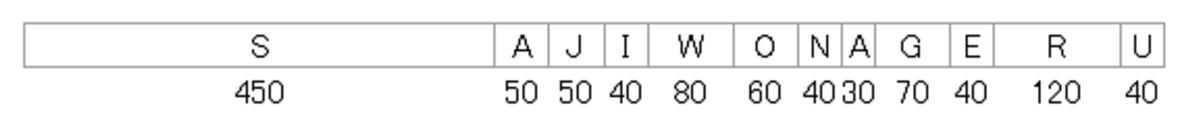
\includegraphics[width=14cm,clip]{res_x_i/ety_bar.eps}
 \end{center}
 \caption{文字ごとの打鍵時間}
 \label{x_i:ety_bar}
\end{figure*}

\answer{精}{見方はわかりますよね。各文字を入力する際にかかった時間が、その部分の横幅に対応しています。数字の単位は ms(ミリ秒、1/1000 秒)ですね。}

\answer{僕}{最初の\key{S}でかすぎだろ、常識的に考えて。}

\answer{精}{初めのキーは\key{S}じゃなくても、どんなキーでもこういう結果になります。打鍵速度が遅いうちは気になりませんが、後ろの部分の打鍵速度がこれくらい速くなっていると、むしろここが重要というわけです。}

\answer{僕}{450ms って……これはどうなの? 遅い方?}

\answer{精}{これも個人差がすごくあるんですが、特に訓練をしていないタイパーで 450ms から 500ms 程度だと思うので、並ですね。今のあなたのレベルだと……平均 500ms 以上はかかるかな。}

\answer{僕}{……でもこれは 100ms とかには絶対ならないよね。反射神経的にさ。}

\answer{精}{訓練すると、平均 400ms に持っていくことは誰にでもできると思います。そして初速・レイテンシを重視して記録を出しているトップランカーともなれば 350ms 程度がバシバシ出せます。数字だと僅かな差に見えるかもしれませんが、ワードが短いと、これだけで 50pt とか 100pt とかの点差につながります。さっきの図、再度凝視してみて欲しいです。後ろの部分はかなり極まってます。ここを速くして 50ms 縮めるのは厳しい。でもレイテンシなら、それくらいは削る余地があります。}

\answer{僕}{もしレイテンシが 350ms になれば全体で 100ms 分短くなるから……割合で見ても相当速くなるね。どうやったら鍛えられるの?}

\answer{精}{一番重要なのは{\bf ローマ字読み}と呼ばれるスキルを身につけること。「\ruby{匙}{さじ}を投げる」の方ではなくて、「SAJIWONAGERU」というローマ字表記された方を読み取って打つんです。}

\answer{僕}{なるほど、「\ruby{匙}{さじ}」を読むのにかかる時間がもったいないってことだ。「S」ならそのまま \key{S} って打てる。でも、一打目はともかく、その先までローマ字読みで速く打てる気はしない……。}

\answer{精}{はじめからローマ字読みをしていたという人もいますけど、訓練で後から身につけることもできます。一朝一夕には無理ですけどね。初めだけローマ字読みして、ワードの半ばからは漢字かな交じり文の方を読む人もいますし。}

\answer{僕}{今すぐは手がでないな……他には?}

\answer{精}{反射神経を鍛えるため、右脳的なトレーニングをすることも効果がありそうです。瞬間的に判断する脳の働きを鍛える感じでしょうか。}

\answer{僕}{それは才能というか、生まれつき決まってるんじゃ……?}

\answer{精}{「反射神経」と言うと、そういう神経があって、生まれつきみたいに思っちゃいますけど、生物学的にそんな神経はないですし、陸上選手だって卓球選手だって、後天的に鍛えてますよね? 才能のような要素がゼロだとは言いませんけど、そう言って逃げちゃうのは最後の手段。まず努力して、考えて、工夫して、また努力して……その後の話です。}

ジーザス、久しぶりに目が怖かったので、僕はそこで納得して、この話はもう持ち出さないようにしようと密かに誓った。

\subsubsection{ワード末尾部分の高速化}

\answer{精}{初めの部分がボトルネックなら、最後の部分は攻める場所です。}

\answer{僕}{後半加速が重要、ってのはさっきも言ってたけど?}

\answer{精}{もっと加速するのです! ワードとワードの間に、休み時間がありますよね。だから、各ワードを打ち切る最後の部分ではかなり無茶な打ち方をしても体制を整え直せる。それを利用して、ワード末尾はあとのことを考えず、手首や腕の動きも使ってドカンと一気に打ち込む……{\bf スパート}と呼ばれたりしますね。}

\answer{僕}{言ってる意味はわかるけど、感覚的にはさっぱりわからない。練習しようもない。}

\answer{精}{ですよねー(←やや嬉しそう)。まあ、基礎能力が一定レベルになったら感覚的に納得できます。その時に使うかどうか検討してください。}

\subsubsection{入力文字数の水増し}

\answer{精}{あとは、レイテンシの話とも関係して、ワードの長さ……結果画面でいう「入力文字数」を増加させる裏技的なテクニックがあります。}

\answer{僕}{前にディープだから後回しって言ってたね。裏技って何事……。}

\answer{精}{e-typing は柔軟にローマ字入力を受け付けてくれるので、わざと打鍵数が多くなるような打ち方をするんです。比較的簡単なのは「し」の \key{S}\key{H}\key{I} や「う」の \key{W}\key{H}\key{U} でしょう。過激なところでは「い」\key{Y}\key{I} や「っ」\key{L}\key{T}\key{U} のようなものまで使う変態もいないことはないです。}

\answer{僕}{\key{W}\key{H}\key{U}なんて、その入力自体初めて知ったっていうレベル。}

\begin{screen}
いっしょう\\
ISSYOU\\
YIXTUSHILYOWHU
\end{screen}

\answer{精}{この例は極端ですが、打鍵数が倍以上になっています。}

\answer{僕}{打鍵数が増えると何か得だっけ? スコアは WPM を元にするから、速度が速くないと意味ないんじゃ。}

\answer{精}{そこでレイテンシが関係するんです。ワードが長くなればなるほど、レイテンシによるタイムロスを後ろの部分の高速打鍵で補うことができますよね。}

\answer{僕}{ん……うーん?}

\answer{精}{「うし」を \key{U}\key{S}\key{I} って 400ms で 3 打鍵できますか?}

\answer{僕}{まず無理……レイテンシだけで 450ms とかになるって言ってたし、その時点で僕には無理。}

\answer{精}{6 打鍵の \key{W}\key{H}\key{U}\key{S}\key{H}\key{I} を 800ms ならどうです?}

\answer{僕}{最初の \key{W} が 450ms くらいで、残りが 350ms ……厳しそうだけど、無理ってほどじゃないのかな。可能性は見えてる。}

\answer{精}{計算するとわかりますが、どちらも WPM は 450 になります。後者の方が楽ですよね。}

\answer{僕}{WPM は「速さ」だから、「道のり」(打鍵数)と時間が両方倍になっても変わらないってことね。}

\answer{精}{{\bf 水増し打鍵}と呼ばれています。わざと長くなるような打ち方をするというのは、タイピングを入力の手段として見ると本末転倒なので、賛否両論ありますし、効果も微々たるもので使わない人も多いですが…… e-typing をゲームとしてみた時にはこうした攻略もあるということです。}

\answer{僕}{ぐぬぬ……。(←気絶寸前)}

\subsubsection{どこまで行っても正確性}

\answer{精}{もちろんですが、以上のような非常に高度なことを行いつつ、正確性は維持しなきゃダメです。打ち始めを高速化し、隙あらば長くなるような打ち方で打鍵数を稼ぎ、各ワード末尾では瞬間的にものすごく加速しながら、ミスはできるだけしない。このような戦いになってきます。}

\answer{僕}{す、数ミスなら問題ないんじゃなかった……?}

\answer{精}{このレベルになると、そうも言っていられません。スコアの計算式、覚えてますか?}

\answer{僕}{WPM から EPM をひいて、正誤率の二乗を……。}

\answer{精}{「かける」。そこが曲者です。スコアが割合で減っちゃうわけです。WPM の 5\% が減らされるとして、WPM が 400 なら 20pt ですけど、WPM が 800 だと 40pt 減ります。}

\answer{僕}{40pt は痛いってレベルじゃないね……ちょっとミスをしただけで、致命傷なんだ。}

\answer{精}{目指すのはあくまでノーミスです。結果的に 1 ミスか 2 ミスくらいで良い記録になることもありますけど。数ミスなんてしちゃったら、基本的にダメですね。}

\answer{僕}{うーん……ちょっと……見えない世界だ……。}

\answer{精}{はい、どう見ても喋りすぎました。今の時点ではこういうことは全然意識しなくて大丈夫。忘れておいて、頃合いになった時にでも、ふと思い出してくれれば十分です。}

どこまでも空は\ruby{禍々}{まがまが}しく、そして\ruby{艶}{あで}やかに\ruby{煌}{きら}びやかに VIP クオリティさえ包括するレベルを目の当たりにし、全力で頭が痛くなった僕は、その日は練習もそこそこに、e-typing 腕試しのランキングを眺めて寝た。

\section{Weather Typing と最適化}
\begin{screen}
もうあの記録が破られることは絶対に無いでしょう。\\
――あきうめ、自身の TOD 日本記録を振り返って
\end{screen}

\subsection{タイピングのモデル化}

その翌日。いつものように昼食を終えるなり図書室に駆け込んでパソコンスペースを占領し画像検索を始めようとした僕の前に、ヤツがにょろっと現れた。

キーボードの上に現れるメカニズムは未だによく解明されていないが、このシュールな光景にもだいぶ慣れつつある。

\answer{精}{暇ですねー。}

\answer{僕}{いや君やることないの!? っていうかずっとストーキングしてるの!? っていうか学校でまで独り言つぶやかせたいの!?}

\answer{精}{タイパー志望ってことは、変態志望みたいなものですからね。}

\answer{僕}{いやこれは変態っていうか変質者だから!}

\answer{精}{さておき、e-typing 練習を通して、とにかく指を速く動かすことができればタイピングが速い、なんてことはないと痛感したことと思います。}

\answer{僕}{あーもう、いきなり説明に入っちゃったよこの人……。}

\answer{精}{人じゃなくて精なんでー。……そんな運動能力のようなものは、一要素に過ぎない。あんだすたんです?}

\answer{僕}{そりゃまあ、指を速く動かすだけなら、こうやって、がちゃがちゃがちゃって適当に打てばめちゃくちゃ速いもん。でも実際はこのスピードでは打てない……ワードを読んで、正しく打たなきゃいけないから。}

\answer{精}{実はその「読む」「打つ」をもっと詳しく掘り下げたモデルが考えられていますので、ここで簡単に解説したいと思います。この先の話をするのに便利なので。}

\answer{僕}{モデルとかリア充は爆発してよ……。}

\answer{精}{「モデル」というのは目に見えないようなことを説明しやすくするために、考え方に簡単な形を与えたもの……のことです。まず、タイピングをする際に行われているステップを大きく三つ、{\bf 認識} {\bf 組立} {\bf 動作}に分解して考えます。}

\answer{僕}{ちょっと待った。僕は今、子守歌を四時間にわたって拝聴し、お腹の中を山の幸で満たし、四月の陽気に包まれて、この静かな図書室で香り立つようなふかふかのソファーに全体重を預けている。君の解説を聞いて、寝ないことがあるだろうか? いやない。}

\answer{精}{意外と寝ないと思いますよ。むしろ e-typing で苦労した経験のある今のあなたにとっては、エキサイティングなはず。}

\answer{僕}{やれやれだぜ……。(←眉につばをつけている)}

\answer{精}{全力で腰を折られたので再掲しますと、{\bf 認識} {\bf 組立} {\bf 動作}に分けます。第一のステップは「認識」です。ワードを視覚などでとらえて、今から打つべきはどういう文章なのか、と把握するところまでです。}

\answer{僕}{「読む」と同じ?}

\answer{精}{大体そうでしょう。ただ、音を聞いて打つタイピングゲームがあったとすると「読む」では不適切なので、「認識」という言い方になってますね。}

\answer{僕}{それじゃあ、僕の言う「打つ」は「動作」か。}

\answer{精}{そこが難しいところです。「動作」はもちろん、指を実際に動かしてキーを打ちに行くことなんですが……ここで質問タイム。「認識」でどういう文を打つかが判明した時点で、「動作」できますか?}

\answer{僕}{できそうな気がするけど……そんなこと聞くってことはできないんでしょ。三つのステップってさっき言ってたし。}

\answer{精}{……ひきょうものぉ……。でもその通り。「認識」だけでは、どういう文字の並び({\bf 文字列})をこれから入力するか、ということしかわかりません。「動作」するためには、どのキーを打てばいいか、そのキーは物理的にどこにあって、どの指をどう動かせば打てるか……そういうこともわかっていないとだめですよね。そのイメージの集まりに{\bf 打鍵列}と名前をつけます。}

\answer{僕}{「動作」は本当にただ動かす部分だけなんだね。その直前の、どのキーをどの指で打つのか、みたいなイメージ……打鍵列だっけ。それを作る部分は別に必要だと。}

\answer{精}{はい、そのステップの名前が「組立」です。実際に打つイメージを頭の中で組み立てるという感覚ですね。このステップは、ほぼ無意識に行われていることも多いかと思いますが、競技レベルになると必要に応じて意識する必要があります。「認識」「組立」「動作」。こう説明すれば、自然な分け方だと思いませんか?}

\answer{僕}{まあ……(いいように誘導されてる気がするけど)そうかな。僕たちは実際こういうステップで打ってるってこと?}

\answer{精}{厳密な意味では、違うでしょう。脳とか神経とかのレベルに分解すれば、本当はもっと山のようにステップがあるはずで。ただ、私たちにとってちょうど考えやすく、それなりに細かく分析もできるので、今はそういうものだと思って考えましょうというお話です。}

\answer{僕}{まだ全然、どう役に立つのかわからないよ。}

\answer{精}{個々の要素を説明してる段階ですからね……最後に合わさると、すごいです。もうひとつだけ下準備をさせてください。{\bf バッファ}というものを導入します。}

\answer{僕}{(ややカッコイイのが出てきた……)}

\answer{精}{難しい単語に見えますが、大したことはないです。上にも下にも栓がついているペットボトルを考えてください。上から水を入れると中に水が溜まり、溜まった水は下の栓を開けると外に出すことができる。そういう一時的に水をためる装置にバッファという名前がついていると思えばいいです。}

\begin{figure}
 \begin{center}
   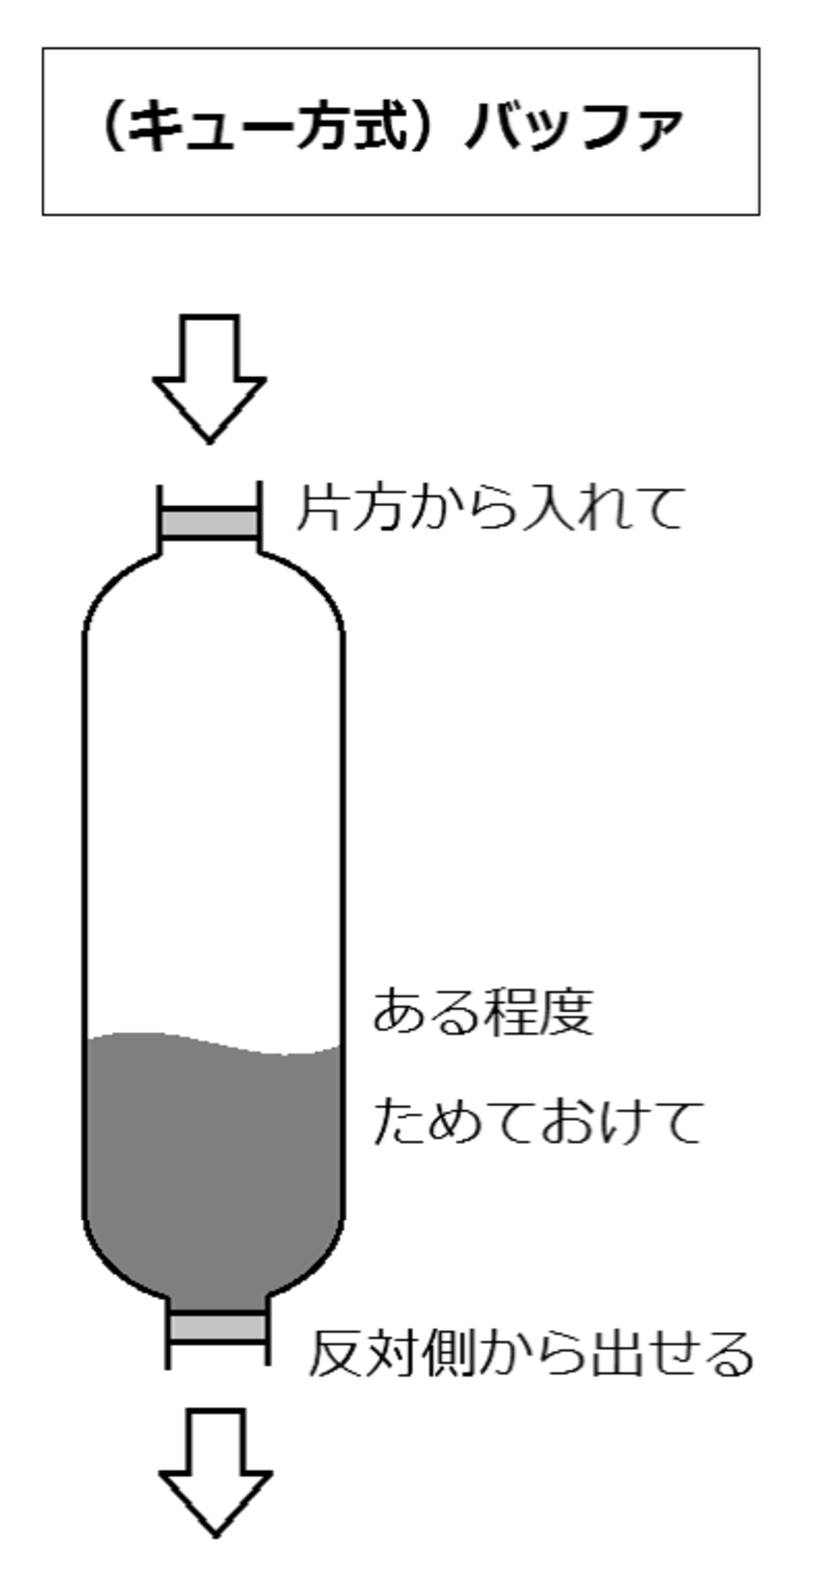
\includegraphics[width=7cm,clip]{res_x_i/model1.eps}
 \end{center}
 \caption{バッファ}
 \label{x_i:model1}
\end{figure}

\answer{僕}{どういうものかはわかったけど……これ何の役に立つの?}

\answer{精}{例えば、上からちょっとずつ入ってくる水をしばらくためてから、一気に下の栓をあけてドバァってやるとか。こういう装置がないとできないですよね。}

\answer{僕}{まあ、そうだけど……。}

\answer{精}{逆に一気に上からドバァって来たのをためておいて、後からちまちま出して使ったり。そういう風に、出し入れの速度を調整するために使えます。}

\answer{僕}{まだ微妙だけど……名前がカッコイイから許した。}

\answer{精}{実際に使われているところを見た方が早いですね。このモデルでは、バッファを縦に二つ、連結します。図をどうぞ。}

\begin{figure}
 \begin{center}
   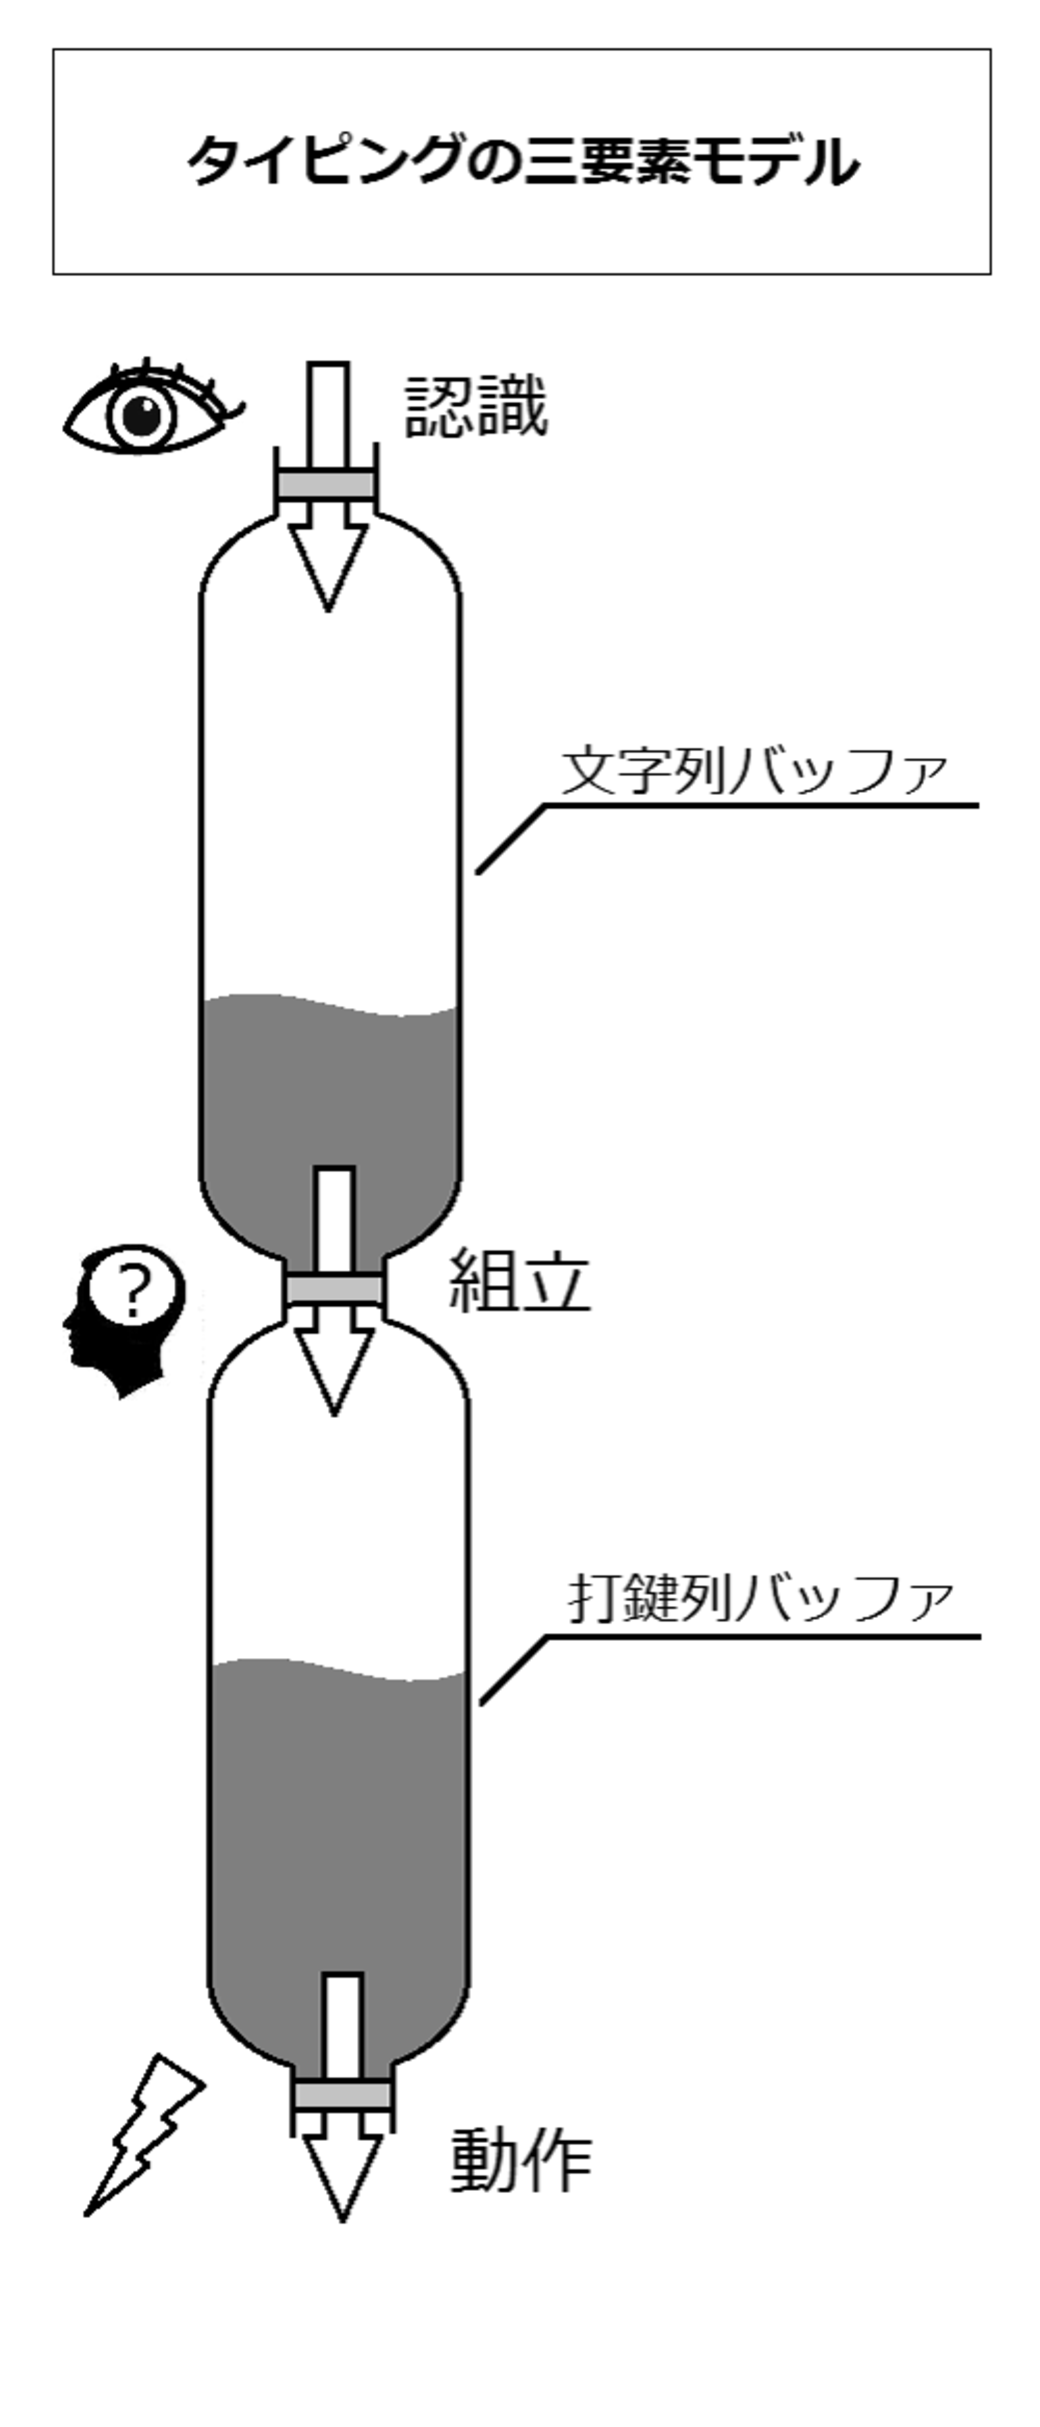
\includegraphics[width=7cm,clip]{res_x_i/model2.eps}
 \end{center}
 \caption{タイピングの三要素モデル}
 \label{x_i:model2}
\end{figure}

\answer{僕}{(連結した!?)}

\answer{精}{図を見てもらえばだいたいわかっちゃうと思いますが……まずワードを「認識」すると、こういう文字列だなという理解が、上の文字列のバッファにたまります。}

\answer{僕}{まだ「文字列」だから、どう打てばいいかってことはイメージできてないわけだね。}

\answer{精}{そうです。「認識」しただけでは打てないので、続けて「組立」です。文字列バッファに溜まっている水(文字列)から一定量取り出して打鍵列を「組立」するわけですね。できた打鍵列が下の打鍵列バッファに溜まります。}

\answer{僕}{おお……。}

\answer{精}{打鍵列が完成したらめでたく「動作」できます。つまり「動作」では打鍵列バッファから水(打鍵列)を取り出して、実際の打鍵を行うことになるわけです。どうですか!}

\answer{僕}{バッファの役割がわかった気がする。}

\answer{精}{大事なポイントとしては、「認識」「組立」「動作」はそれぞれ順番に行われるわけではなくて、同時並行的に進めることができるってことです。}

\answer{僕}{それぞれの栓を同時に水が通過していけるイメージね。}

\answer{精}{そして私たちがやっている競技は、このモデルで言うと、ワードという一定量の水をこの装置の上から注ぎ込んで、どれだけ早く一番下まで\ruby{濾過}{ろか}完了するかという勝負なわけです。}

\answer{僕}{今まで「読む速度が遅い」と言ってたのは「認識」「組立」部分の栓が細いってことで……「打鍵するだけならいくらでも速くできる」って言ってたのは「動作」の部分の栓は他と比べると太いってことだ。}

\answer{精}{考察しやすそうでしょう? e-typing でワードの初めの部分で急ぎすぎるとミスしやすいという話がありましたが、あれは「認識」「組立」が追いついてなくて打鍵列バッファが空なのに、無理に「動作」しようとしたからなんです。}

\answer{僕}{早すぎたんだ……打鍵列が腐ってやがる、と。モデルがあると便利ってこういうことね!}

\answer{精}{これからは、このモデルの理解を前提に話をしますね。}

\subsection{動作がネックになる時}

帰宅後、早速今日得た情報を使って e-typing を攻略しようとしたところ、タイピングの妖精さん(←そういうことで妥協したらしい)に止められてしまった。

\answer{精}{せっかく三要素モデルを紹介したので、「動作」の部分がつらいケースも知って欲しいのですよ。}

\answer{僕}{「動作」は大丈夫だ問題ない、でファイナルアンサーなんじゃなかったっけ。}

\answer{精}{e-typing に取り組む分には、まだしばらくそうです。でも世の中には他の競技種目となるタイピングゲームもあるので。そろそろ他のものも紹介したいと思って。}

\answer{僕}{ぶっちゃけ e-typing のミス音と血しぶきに殺意を感じ始めてたから、嬉しいな。}

\answer{精}{Weather Typing というのが「動作」の限界を感じるには良いので、ダウンロードしてきて下さい。}

\answer{僕}{インストールは僕に任せろー! ……オーケー、あとは WeatherTyping.exe を起動して、と……「シングルプレイ」でいいの? ってか対戦もあるんだね。}

\answer{精}{対戦についてはここでは詳しく解説できないですけど、よく出来ていて楽しいですよ。Weather Typing に慣れてきたらぜひ挑戦してみてください。}

\begin{screen}
Weather Typing\footnotemark

本当はネット対戦がアツくてメインなソフトなのですが、この記事ではシングルプレイに限定した書き方になっています。
対戦にも興味を持たれた方は、上記ページの「その他」→「ロビー」→「参加方法」を参考にロビーに入って常駐するといいでしょう。
ただ最近は常に人がいるという状態ではないようなので、友達を誘うと確実です。
\end{screen}
\footnotetext{\url{http://denasu.com/software/weathertyping.html}}

\begin{figure}
 \begin{center}
   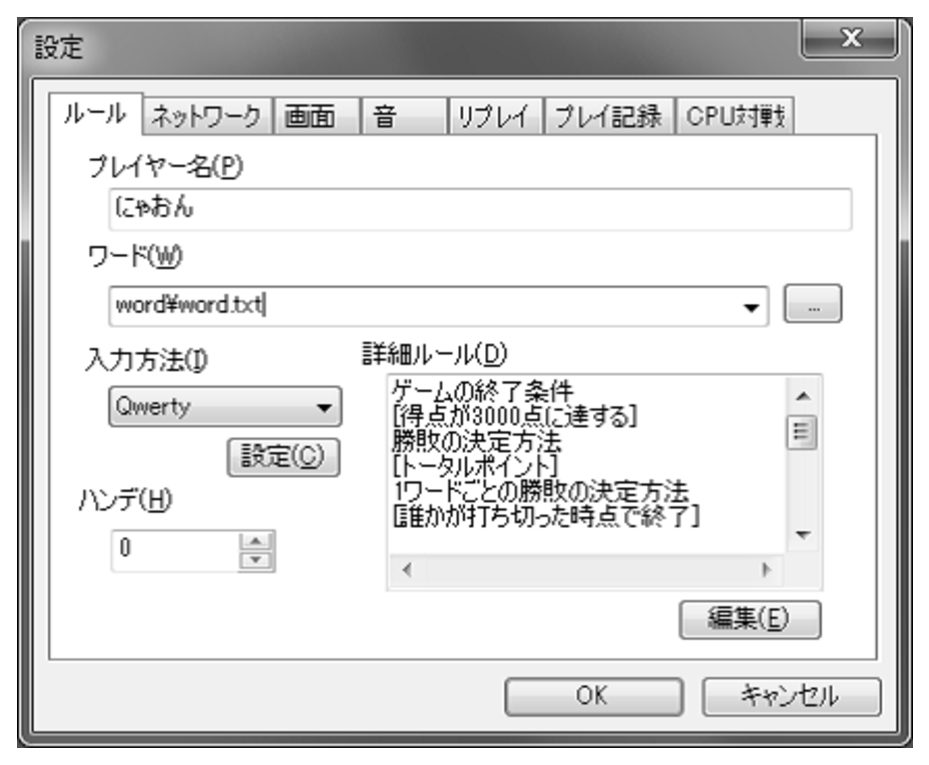
\includegraphics[width=7cm,clip]{res_x_i/wt_setting.eps}
 \end{center}
 \caption{Weather Typing 設定画面}
 \label{x_i:wt_setting}
\end{figure}

\answer{僕}{たくさん設定項目が出てきたけど……。}

\answer{精}{かなり細かく設定ができるんですけど、重要なものはあまり多くないです。今はとりあえず「ワード」とある欄でワードファイルを指定できるということだけ覚えておきましょう。}

\answer{僕}{ワードを自分で作れるんだ。}

\answer{精}{e-typing に慣れていると新鮮ですよね。だから e-typing のワードで練習したいものだけ集めてきて Weather Typing で練習したりなんてこともできます。今はデフォルトのワードファイル word.txt のままでやってみましょう。}

\begin{screen}
独自のワードファイルは直接テキストファイルを編集して作るか、Weather Typing 本体に\ruby{同梱}{どうこん}されている WordMaker.exe を使って作ります。
WordMaker.exe を使えば簡単に作れますので、一度やってみることをおすすめします。
\end{screen}

カタカタカタ。

基本的には e-typing と同種のゲームという感覚だ。画面にワードがひとつずつ表示されて、打ち終わると次のワードに行く。独特のワードに所々つまずきつつも、順調に打つ。……やや長い。

\answer{僕}{……終わった。Complete 30、Speed 510、Accuracy 92 で、Total が 46920。}

\answer{精}{結果の解説は要ります?}

\answer{僕}{いや、もう大体わかる…… Complete はワード数、Speed は e-typing の WPM と同じ意味で、分速何打鍵か。Accuracy は正誤率。Total がスコアでしょ。}

\answer{精}{ばっちりです。ちなみに Total は Speed かける Accuracy で計算されてますよ。}

\answer{僕}{e-typing はスコア計算でミスが三重ペナルティだったから、それに比べるとミスのペナルティは小さいな。}

\answer{精}{Weather Typing の方がスピード重視ですね。ですが、Weather Typing でスコアアタックをする際に一番大切なポイントは、そんな部分じゃないんです。}

\answer{僕}{一番大切なポイント……(ごくり)。}

\answer{精}{Weather Typing では、e-typing の章で解説した初打までの時間「レイテンシ」が、なんと計算に入りません。}

\answer{僕}{計算に入らない? ……ワードが表示されてから、ゆっくり考えて打ってもいいと?}

\answer{精}{イエス。なので、基本的な部分では e-typing に対する攻略が流用できますけど、上級レベルになると e-typing とは別ゲーになります。何しろ短いワードなら最初にじっくり見ておくことで「認識」「組立」を完全に完了できます。つまり打鍵列バッファが満タンの状態で、あとは「動作」だけという所からスタートして競えるわけです。}

\answer{僕}{どれだけ指を速く正確に動かせるかって勝負……。}

\answer{精}{このように打鍵列を十分に組み立ててから一気に打つことを、{\bf ため打ち}と言ったりしますね。}

\answer{僕}{ゲーム的で面白そう。}

\answer{精}{もっと面白くするために、このワードファイルで打ってみるといいです。}

\begin{screen}
ダウンロードして頂けるようにワードファイルを置いておきます。\\
\url{http://dvorak.jp/archive/bura.txt}

Weather Typing のフォルダ内にある word というフォルダの中に保存し、Weather Typing 起動時の画面でこの bura.txt を選択すると使うことができます。

ちなみに、以下の 20 ワードが入っています。

あみあみ かにかに きらきら くいくい\\
くらくら こうこう これこれ さくさく\\
ざわざわ たじたじ ぬくぬく ぬるぬる\\
ふらふら ぶらぶら ぶんぶん ちょこちょこ\\
ぽきぽき むんむん ほげほげ しゅいしゅい
\end{screen}

\answer{僕}{いかにも打ちやすそう……しかも、考えてから打ってもいいと来た。いくらでもスピード出せるでしょ!}

\answer{精}{そう思いますよね。でも実際は……ま、いつものパターンです。}

\answer{僕}{そうわかっていても、突撃するのが僕だった! スタート、っと。}

「くらくら」……えーと\key{K}\key{U}\key{R}\key{A}……楽勝。「さくさく」……楽勝。「ぶんぶん」……人差し指が……。「むんむん」……うーん、きつい。「ざわざわ」……フォオオオ!

\answer{僕}{…… Speed 670。ワードが短いし、レイテンシ無視で考えてから打てるから、さっきより断然速くはなってる。けどワードによっては全然だめだったな。「むんむん」とか。}

\answer{精}{「ぶんぶん」「ぬるぬる」「むんむん」「ぬくぬく」あたりは右手の人差し指を酷使するワードですね。}

\answer{僕}{そいつらはまだいいとして……「ぽきぽき」「ざわざわ」は指がつるかと思った。これが「動作」がボトルネックになる感覚……。}

\answer{精}{その一部ですね。これだけお膳立てすれば「認識」「組立」が十分なレベルでなくても、「動作」もいずれ問題になりそうだということが体感できたでしょ。そして、もっと速くなると e-typing のような競技でも、部分的にボトルネックが「動作」になることはよくあります。}

\answer{僕}{「動作」は物理的な指の動きだから……指を鍛えたりすれば伸ばせるよね。}

\answer{精}{頑張って競技タイピングをやっていると、タイピングに関しては、どんどん指が器用になっていきますね。キビキビと正確に動くようになります。}

\answer{僕}{今までは先読みだとかノーミス意識だとか、脳トレ的な話ばっかりだったけど、筋トレ的な要素もちゃんとあるんだね。}

\answer{精}{タイピングは頭も身体も使う万能競技ですよ。ダイエットにも(多分少しは)なります。}

\answer{僕}{手とか指しか動いてないけど?}

\answer{精}{それでも、二、三時間も本気で打てば汗だくになれます。それくらい激しく「動作」できるくらいに、他の部分が速くなってからの話ですけどね。}

\answer{僕}{タイピングで汗だくは想像したくない……。}

\subsection{打ち分け・最適化}

何度も例のワードファイルで Weather Typing を打っていると、どんどん指の動かし方に慣れてきた。速いワードはとことん速く、遅いワードも詰まらないように。動作部分の訓練は、どうやら僕に向いているらしかった。

\answer{僕}{よし! Speed 750 突破ッ!}

\answer{精}{わあけっこうすごいですねー(←上から目線)。}

レイテンシを無視しているとはいえ、e-typing で 750pt といったらトップレベルだ。これくらいのスピードで e-typing のワードを打ち続けることができれば、750pt ……!

僕はタイピングを始めてから最大級の胸の高鳴りを覚えていた。

だから、こんな挑発をしてしまう。

\answer{僕}{ヨウセイサァン、余裕じゃないっスか……これの記録どんだけなんスかぁ?}

\answer{精}{私ですか?}

\answer{僕}{そっスよ……最初の一回 e-typing 見せてもらってから全然手本見せてくれないじゃないっスか。}

\answer{精}{それは……教育上よくない理由がありまして。でも良い頃合いですね。見せましょう。多分、2000 とか出ますけど。}

\answer{僕}{2000!?}

さすがに冗談だと思った。

―― 二分後 ――

\answer{僕}{ォオオオオオオオオオオオオ!!!}

ワードが爆風に飛ばされるように消えていく……。まさに瞬殺。打ち始めたと思った直後には、すべて打ち終わって、消えている。

そして彼女に乗っ取られた僕の手が、僕の指が、変な方向に曲がって奇妙な動きを見せている。なんだこれは! 大丈夫なのか!? 異次元パワー\ruby{炸裂}{さくれつ}しすぎだろ常考ッ……!?

\begin{screen}
ワードは違います(この動画の方が遥かに高度です)が、参考動画をどうぞ。
ひろりんご氏の独自ワード Speed 1905 Accuracy 100\\
\url{http://youtu.be/jf9kArBHQvE}
\end{screen}

そして打ち終わる。

\answer{精}{……うーん…… Speed 1700 でした。残念、2000 行かなかったですね。まあ「ざわざわ」出すぎでした。運ゲー運ゲー。}

\answer{僕}{ちょ、ちょっと……これは\ruby{卑怯}{ひきょう}っスよ先生……異次元パワー使ってるじゃないスか!}

\answer{精}{はい? ……ああ、手の角度とかの話ですね。}

\answer{僕}{なんなんだこれ……なんなんだこれ……。}

\answer{精}{これが教育上よくない理由そのものです。{\bf 最適化}などと呼ばれています。}

\answer{僕}{やっぱり長門有希的大宇宙能力じゃないっスか!}

\answer{精}{違いますからね……。最適化というのは、ワードに応じて打ちやすいローマ字を選択したり、打ちやすい指で打つように標準の運指を崩したりする技術のことです。前者は{\bf 打ち分け}、後者を{\bf 最適化}として言葉を分ける一派もありますね。}

\answer{僕}{ローマ字を選択? 運指を崩す?}

\answer{精}{えーと……ひとつずつ行きましょう。ローマ字の選択の方の「打ち分け」ですが、これについては e-typing の時に近いことを少しやってます。覚えてませんか?}

\answer{僕}{あれか、水増し打鍵――「う」を \key{W}\key{H}\key{U} で打つみたいな。}

\answer{精}{それそれ。あの時は、打鍵数を増加させるために普通と違う打ち方をするという話でした。今度は、打ちにくいパターンを避けるために使います。}

\answer{僕}{例えば?}

\answer{精}{{\bf C打ち}が代表的なのでこれで解説しましょう。これは「か」「く」「こ」を入力する時に\key{K}ではなく\key{C}を使うテクニックで、打ち分けの一種ですね。}

\answer{僕}{別に\key{K}でも\key{C}でも変わらない気がするけど……。}

\answer{精}{その部分だけ見たらそうです。でも前後のパターンと合わせると……。今回のワードですと「かにかに」「くいくい」「こうこう」「ぬくぬく」「ちょこちょこ」はC打ちによって劇的に打ちやすくなります。}

\answer{僕}{\key{C}\key{A}\key{N}\key{I}、\key{C}\key{U}\key{I}、\key{C}\key{O}\key{U} ……本当に一瞬で打てるような動きに変化した。}

\answer{精}{私は「ちょこちょこ」は CHOCO と打ちますね。速く打つのは、他と比べるとちょっと難しいですけど。}

\answer{僕}{「ぬくぬく」もわからない。\key{C}にしてもあんまり変わらないような。}

\answer{精}{これは運指を崩す方の最適化と合わせて考えないといけないですね。こっちは要するに、このキーはこの指で打ちましょうという原則的なルールを破ることです。}

\answer{僕}{ルールを破る……。}

\answer{精}{そうです。確かにタッチタイプを学ぶ段階ではホームポジションを守り、一般的に教えられる通りにキーごとに担当する指を固定する(標準運指)方が習得が楽でしょう。でもそれって別に、打てるようになった後は破ってもいいですよね。指が動ける範囲はもっと広いので。}

\answer{僕}{タッチタイプってレベルじゃねーぞ! そこまでやるの……恐ろしい……。}

\answer{精}{一例ですが、私は「ぬくぬく」なら\key{N}を人差し指で打った後、\key{U}を中指で打ちます。標準の運指ではないですけど、手の角度的にかなり打ちやすくて自然にいけると思います。そして「く」は右手中指を\key{U}に置いたまま\key{C}\key{U}ですね。こうすると\key{N}\key{C}\key{U}すべて別の指が担当することになって、かなり速いです。}

\answer{僕}{本当だ、\key{U}を中指で打つのは手首をひねる感じで打つと……意外に自然。それでさっきは、手があんな奇妙な動きをしてたのか。}

\answer{精}{そういうことです。今回の他のワードだと「ぬるぬる」「むんむん」「ぶんぶん」にも応用できますね。}

\answer{僕}{「ふらふら」「ぶらぶら」「しゅいしゅい」あたりは?}

\answer{精}{最適化というのは個人個人でやり方に差がありますし、自分でも考えてみるといいんじゃないでしょうか。基本的な方針としては、同じ指を連続して使わないで済むようにすると、たいてい速い運指ができあがります。}

\answer{僕}{「しゅいしゅい」は\key{Y}を左手人差し指で……こうかな? いや、でも「しゅ」\key{S}\key{H}\key{U}にすれば右手で一気に行ける……こっちの方がいいかな……。}

\answer{精}{奥が深いですよね? 最適化に関する議論は、現役タイパーの中でもまったく終わっていないです。各運指を習得するコストや、「組立」の段階で最適化を検討しなければいけないコストを気にして、やらない人もいますし。あまり早い段階からこういう小手先の技ばかりに気を取られるのもどうかと思って、もったいぶってきましたが……今のあなたなら制御できる力でしょう。}

\answer{僕}{うーん(←聞いてない)、「ぽきぽき」はどうやるの?}

\answer{精}{それはもう、左手を右手範囲まで持っていって手伝うんです。}

\answer{僕}{KIMEEEEEEEEEEEE!!!}

\answer{精}{さすがに Weather Typing でこういうワードを打つとき限定ですけどね。他のゲームで出てきたら、普通にぽきぽきした方がいいです。それか \key{P}\key{O}\key{K}\key{I} \finger{9877}。}

\answer{僕}{しかし「ざわざわ」に至ってはもう、どうしようもないね……。}

\answer{精}{(うわーやっぱり最適化ハマっちゃいますか)そういう場合もありますね。}

\answer{僕}{どうしよう?}

\answer{精}{どうもこうも、さっき自分で言っていた通り、指の動きを速くすればいいじゃないですか。最適化の考え方に慣れすぎると、最適化できないパターンは諦めてしまいがちです。でも実は、指を鍛え、運動を洗練させて、打鍵を速くする余地は十分にあるわけです。その基本に立ち返ることも、時には大事ですよ。……と釘を刺しておきますね。}

\answer{僕}{うーん(←全然聞いてない)、ざわざわ……ざわざわ……。}

たかがタイピング、されどタイピング。つくづく底の知れない世界なのだった。

五年後、手を交差させる超絶変態運指「グランドクロス」を完成し、競技タイピング界に大旋風を巻き起こすことになるとは――この時の僕には知る由もない。

\begin{screen}
「精」が釘をさしていますが、他でもない私がそのパターンで長年記録が伸び悩んだ人だったりします。最適化を使うと、ちょっと考え、ちょっと練習すればそのパターンがすぐ速くなるのでハマりがちですね。実際とても楽しいですが、行き詰まりを感じた際には、地道な訓練も大事だと思い出しましょう。

なお、最適化でも対応に困る「ざわざわ」のような文字列をも打ちやすくする、まったく別のアプローチも実はあります。それは、キーボード配列から変えてしまうこと。
一般的には QWERTY と呼ばれる配列でローマ字入力をしますが、タイパーの中には高速打鍵に向くような別の配列を利用して競技に参加している人もいます。ある意味、最適化よりもさらに前衛的なアプローチと言えるでしょう。
詳しくは、配列について詳しく書かれている他の記事を参照してください。
\end{screen}

\section{タイプウェルの登竜門}
\begin{screen}
無能! 死ね!\\
―― dqmaniac, 己の打鍵失敗に憤って
\end{screen}

\subsection{国内最強ランキング}

タイピングのモデルを知り、最適化や打ち分けを知り、自分で攻略法を考えながら打ち込むことができるようになって以来、タイピングに対する情熱はますます燃え上がった。練習量は倍になり、スキマ時間に最適化について考えるようになり、授業中など暇さえあれば指のストレッチをする。

当然の結果として、成長もすさまじかった。e-typing で 500pt の壁を打ち破るとほぼ同時に Weather Typing の word1 で Lv6 (60000 点)到達。最適化練習のワードでは Speed 1400 が安定して出せる。

e-typing 腕試しのランキング 1 ページ目に自分の名前が載っているのを見てはニヤつく毎日――そんなある日のことだった。

\answer{僕}{この「タイプウェル」っていうのは……なんだろ?}

e-typing のランキングに、その名前を見つけてしまう。

\answer{精}{みつ……けて……しまったん……ですね……。}

おどろおどろしい声色を響かせながらキーボードからお人形的上半身が生えてくる。もちろん、今更驚きはしない。

\answer{僕}{ちょっと待ってよ。まだ隠し事があったの?}

\answer{精}{紙面……構成の……都合……。}

\answer{僕}{なんでもいいけど、そのテンションやめよう、つまんないんで。}

\answer{精}{はーい(←キーボードから飛び出た)。タイプウェルというのは国内で最もレベルの高いランキングを持つ競技タイピングソフトです。現代でも最もメジャーな競技ソフトと言ってもいいでしょう。}

\answer{僕}{国内で最もレベルが高い!? e-typing が最大最強って言ってた気がしまくりんぐですが。}

\answer{精}{日常的な参加者数では、e-typing ですよ。でもタイプウェルのランキングサイト GANGAS では、もう 10 年以上にもわたって記録が蓄積されているんです。e-typing のようなリセットはありません。}

\answer{僕}{10 年……だと……。}

\answer{精}{それも、GANGAS に登録されるのはその人の最高記録。色々なタイパーが――あらゆるタイピング界の偉人が、かつてトップだったタイパーが、伸び盛りの現役勢が――何年もの年月を積み重ね到達点として出した、至高の最高記録! それが何百・何千と集められているこのロマン! わかりますか!?}

\answer{僕}{わかりますッッ!!!}

\answer{精}{よろしい! 突撃です!! 大海があなたを待っている!!!}

\begin{screen}
GANGAS - Type Well Fan\\
\url{http://www.twfan.com/}

本体の入手はページ下部の「概要・ダウンロード」からどうぞ。
\end{screen}

\answer{僕}{僕のブラウザが火を噴いた!}

\answer{精}{タイプウェルの文化はそれだけでかなり深いものがあるので、ページを一見しただけでは何がどうなっているのかわからないですよね。}

\answer{僕}{なんか盛り上がってるということはわかる……「国語R」「国語K」「英単語」「オリジナル」っていうのが種目の名前かな?}

\answer{精}{そこから説明するのがよさそうですね。実はそれらは、それぞれ別のソフトです。}

\answer{僕}{同じタイプウェルなのに?}

\answer{精}{exe ファイルが別、と言えばわかりますかね? ひとつのソフトに全部の種目が入っているんじゃなくて、それぞれ別のソフトになっています。「国語R」はローマ字入力で日本語を打つソフト、「英単語」は英単語を打つソフト、「オリジナル」はランダムな数字みたいな、日本語でも英語でもないような独特のワードを打つソフトです。}

\answer{僕}{「国語K」は?}

\answer{精}{ローマ字入力ではなくて、かな入力で日本語を打つソフトですね。今あなたが打っている QWERTY 配列を使ううちは、お世話になることはないです。}

\answer{僕}{じゃ、とりあえず 3 つをやればいいんだ。}

\answer{精}{ところが、これらのソフトそれぞれに 4 つのモードがあります。}

国語 R
\begin{itemize}
 \item 基本常用語 (常用)
 \item カタカナ語
 \item 漢字
 \item 慣用句・ことわざ(慣こと)
\end{itemize}

英単語
\begin{itemize}
 \item 基本英単語 1500(基本)
 \item 拡張基本英単語 A-F(A-F)
 \item 拡張基本英単語 G-P(G-P)
 \item 拡張基本英単語 Q-Z(Q-Z)
\end{itemize}

オリジナル
\begin{itemize}
 \item 小(大)文字のみ(のみ)
 \item 大文字小文字混在(混在)
 \item すべてのキー(すべキー)
 \item 数字
\end{itemize}

\answer{僕}{圧倒的なボリューム! これ全部別のゲームってこと?}

\answer{精}{ソフトによって打鍵数や表示形式など、細かな点が違ったりはしますが……基本的にはワードが違うものがこれだけある、って認識でオーケーです。}

\answer{僕}{ワードは e-typing みたいに週で変わったりはしないんだよね。}

\answer{精}{本体のバージョンアップで若干の追加・削除が行われたりはしましたが、基本的に変わりません。同じワードが過去から現在に至るまで打ち込まれてきたということです。}

\answer{僕}{燃えてきたよぅ……説明聞いてる場合じゃねぇ!}

\answer{精}{(こんな性格だったっけ……)}

自信があるのはもちろん今まで練習を重ねてきたローマ字日本語入力。タイプウェル国語Rをダウンロード、解凍、そして速攻実行。

\answer{僕}{行くぜ! ……ってあれ、詰まった。なにこれ。}

\answer{精}{ワードとワードの区切りで \key{Space} を押さないといけないんです。}

\answer{僕}{そういうのもあるのか! 任せて!}

カタカタカタカタ……。

\answer{僕}{先生出ました! ダブルエス!! レベル SS 出ました!!!}

\answer{精}{おめでとうございまーす。}

\answer{僕}{はぁ……はぁ……これ疲労すごいよ。長いし……ずっと打ちっぱなしじゃん。}

\answer{精}{e-typing や Weather Typing とは毛色の違う競技ですね。レベルやランキングがタイムだけで決まる点も異色です。ミス数とか関係ありません。とにかく速さ命! っていう、とんがった競技ですね。}

\answer{僕}{ミス 30 もあるけど……初っ端から SS 来たんで、賢者モードぉ。}

\answer{精}{……現実を突きつけるようで申し訳ないですけど、タイプウェルのレベルは基本的にこれだけあります。大区分として無印・S・X・Z があって、それぞれの中に J-A のような小区分がある、と読み取ります。}

\begin{figure}
 \begin{center}
   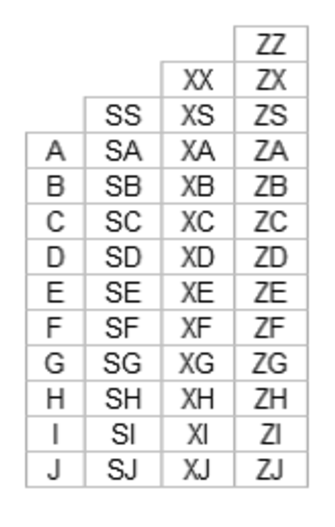
\includegraphics[width=5cm,clip]{res_x_i/tw0.eps}
 \end{center}
 \caption{レベル一覧}
 \label{x_i:tw_level}
\end{figure}

\answer{僕}{僕は SS だから……中間程度!? e-typing 1 ページ目常連のこの僕が!?}

\answer{精}{スペースを押すのにも慣れていない状態で初見常用 SS なら、それなりだと思いますよ。慣れたら X の半ばから X の上の方くらいまではすぐ行けると思います。}

\answer{僕}{XE とかってこと? それってレベル的にどうなの?}

\answer{精}{どこに出しても恥ずかしくないタイパーだと思います。ただ、上には上がいる世界なので……さっきの GANGAS のページからランキングを見てみるといいんじゃないでしょうか。}

\answer{僕}{Z ばっかりじゃん……どこだよ、どこだよ XE ……オウフ、一番下ですか……1000 位とか……。}

\answer{精}{今の記録と比べるなら、SS というと 50 秒以上かかってますから……トップレベルの人は倍以上速く打っていますね。}

\answer{僕}{レベル高すぎワロエナイ。}

\answer{精}{同じワードを何年も打ち込んだりしているわけですしね。打ち切り回数(最後まで打ってタイムを出した回数)も千とか万とかの世界です。e-typing のようなペラペラのランキングとは違うんですよ。10 年積もり積もった結果ですから。日々ランキングを励みにコツコツ記録を伸ばしていって、いつかは憧れの 50 位以内(一番上の枠)に……! と、こういうスタンスで見るものです。}

\answer{僕}{やる気はあるつもりだったけど、ちょっと気が遠くなるかも……。}

\answer{精}{まだまだ伸び盛りですし、心配は要りません。今の自分のレベルより一つ上を目指し、もう一つ上を目指し……とやっている間に、いつの間にか成長しているものです。}

\answer{僕}{ステージをひとつずつクリアしていくって感じなのね。}

\answer{精}{まさにそれです。ランキングに関して、ちょっとモチベーションになりそうなことも言いましょうか? 国内にはこれ以上ハイレベルなランキングは存在しないので、ここで 100 位になれば、かなり堂々と全国 100 位を自負できます。というか国内歴代 100 位ということなので、現役タイパーの中でなら間違いなく 100 位以内と言えるでしょう。}

\answer{僕}{それは嬉しいな。}

\answer{精}{ちなみに、各ソフトのランキングは「総合ポイント」という得点のようなもので競われています。}

\answer{僕}{何がポイントになるわけ?}

\answer{精}{4 つある各モードの自己最高記録のタイムです。まず各モードごとに、タイムに応じたポイントが計算されて、その総和がそのソフトの「総合ポイント」です。}

\answer{僕}{最高記録以外はポイントにはならないのか。}

\answer{精}{ちょっと極端ですよね。でも、だからこそ自己最高記録をどんどん伸ばそうと必死になるわけです。}

\answer{僕}{みんな、こんなに頻繁に自己最高記録を更新してるってこと?}

\answer{精}{そうです。現役競技者のハングリーさはものすごいですよ。ぜひ影響を受けて、少しずつでも記録を伸ばせるようがんばってみてください。}

\answer{僕}{まだわからない部分が多いけど……とりあえず打ってみて、ランキングに参加していればいいんだね。}

\answer{精}{まずはカンペキでしょう。……ランキングについては、本当はもっと色々紹介したいですが……自分で見て回って色々感じて欲しいので、この辺にしておきますね。}

\begin{screen}
なおランキングの参加方法ですが、各タイプウェルの中から記録がコピーできるので、それをメールで送ると、毎週土曜日に反映されます。即時反映でない点も面白いところです。目立った更新だった場合はトップページで紹介されることも。

参加方法について詳しくは、GANGAS 公式の解説\footnotemark を熟読してください。
\end{screen}
\footnotetext{\url{http://members.jcom.home.ne.jp/gangas2/entry.html}}

\subsection{使い方}

全タイプウェルをせっせとインストールした僕。わざわざ全部インストールしたのを見届けた後に、あっけらかんと彼女はこう言う。

\answer{精}{タイプウェルは基本 4 種類あるという話をしましたけど、今からは国語Rに限定して話を進めます。}

\answer{僕}{OH!? タイプウェルオリジナルという謎のソフトに心惹かれてるんだけど?}

\answer{精}{タイプウェルの活用の仕方を身につけて欲しいと思うんですけど、国語、英単語、オリジナルそれぞれ仕様が違って面倒なんです。それに、英単語やオリジナルは e-typing や国語 R とはワードが全然違って、完全に別の競技です。今の段階で手を出すのは早すぎますね。英単語やオリジナルもオールラウンドに打てれば、それはすごいですけど……まずは国語Rに専念してタイプウェルという文化そのものに慣れるのをおすすめします。}

\answer{僕}{うー……了解しておくけどさ。}

\answer{精}{まあ、細かい点が違うだけなので、まず国語Rをおさえておけば大丈夫です。応用が利きます。これがタイプウェル国語Rの基本画面ですね。}

\begin{figure}
 \begin{center}
   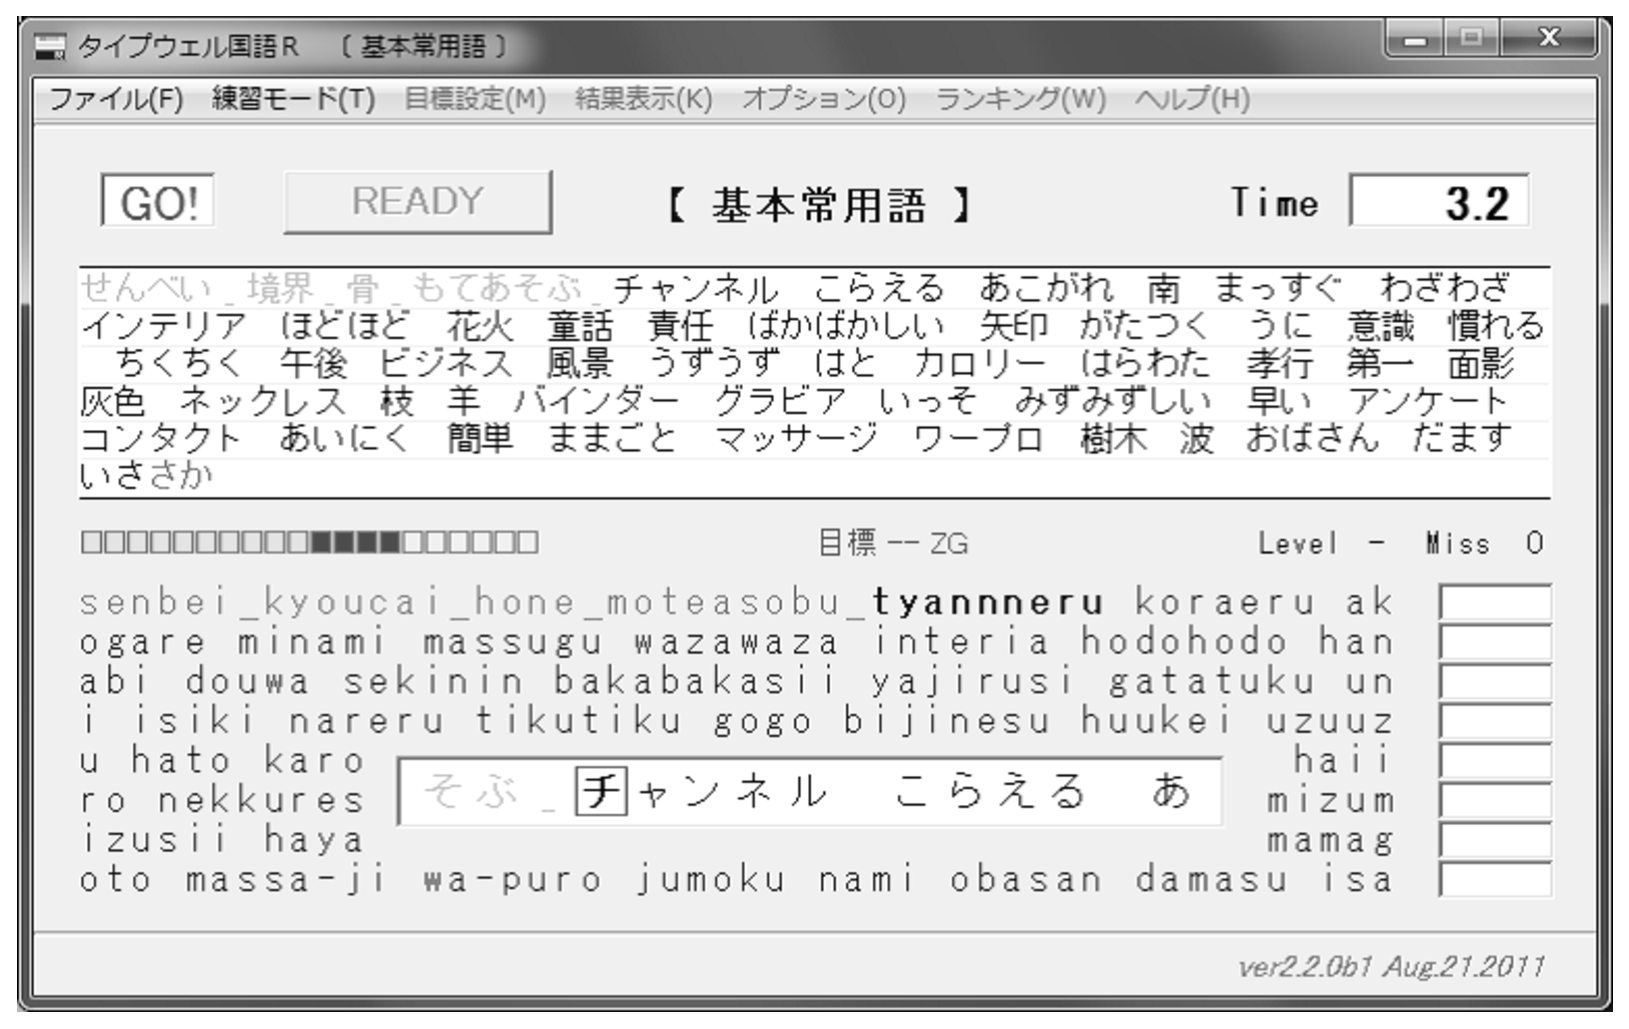
\includegraphics[width=7cm,clip]{res_x_i/tw1.eps}
 \end{center}
 \caption{タイプウェル国語R}
 \label{x_i:tw_mainwin}
\end{figure}

\answer{僕}{機能が詰まってる感じがするよね。}

\answer{精}{言い出せば本当に色々な機能があるんですが、全部解説して、活用法を書き出すとこれだけで本が一冊できちゃうので、タイプウェルプレイヤーなら絶対におさえておきたいポイントを見ていきましょう。}

\subsubsection{基本}

\answer{僕}{この READY っていうボタンをクリックでスタートして……とかそんなことはわかってるから。情強勢甘く見ないでね。}

\answer{精}{いえ、クリックする人は完全に情弱で、普通\key{Space}キーを使います。\key{Enter}でもいいですけど、手をホームポジションに自然に置いたまま、\key{Space}でスタートするのがベターでしょう。}

\answer{僕}{あーそっか。でも e-typing もスペースでスタートだったから、慣れてる。}

\answer{精}{\key{Esc} で中断できるのも e-typing と同じですね。これはある意味一番重要な機能かもです。}

\answer{僕}{……わお、本当に一瞬で中断できる。良い感じに打てるまで何度もこれでやり直せばいいと。}

\answer{精}{そういうスタンスもありますけど、はじめは毎回打ち切る(中断しないで最後まで打つ)ことをオススメします。タイプウェルの特徴のひとつに、記録が色んな面で蓄積されるという点があるんです。だからダメな記録でも、打ち切って蓄積すると……後から嬉しいかもしれません。}

\answer{僕}{他には?}

\answer{精}{先ほども説明しましたけど、各ワードの間に空白が挟まって出題されます。この空白部分では\key{Space}を毎回押さなきゃいけません。}

\answer{僕}{慣れないなぁ、これ……。}

\answer{精}{誰でも最初はそう思うんですけど、慣れてくると親指で\key{Space}を打つのはほぼ完全に無意識になります。なので最初ちょっとイラッとしても、そこは我慢です。我慢して慣れるだけの価値がタイプウェルにはあります、絶対。}

\answer{僕}{右親指で打つか、左親指で打つかは、どっちでもいいわけ?}

\answer{精}{さすが、良いところに気がつきますね。ですが、どちらで打つ人もいて、どちらが有利という結論なんてのは出ていないです。なので、どっちでも良い感じなのですが……ただ、後から変えるのはかなり大変なので、自分で納得した方で打つようにしてください。}

\answer{僕}{そんなこと言われても、余計困るよ。}

\answer{精}{うーん、完全に個人的な意見でよければ、左を薦めます。右手は\key{N}\key{M}周りでの最適化があったり、\key{-}\key{p}など遠目のキーが多かったりするので、左親指を使う方がわずかに有利なんじゃないかと。最適化をしない標準運指スタイルですと、また違ってくるんですけど。また、多くの人は右利きなので、右で打つ方がいいのではという意見もあります。結局、合う・合わないで決めるしかないでしょうね。}

\answer{僕}{うーん……。}

普段のタイピングでも左親指を使っていた僕は、少し悩んだあと、やはり左で打つことに決めた。こういうのは勢いだ。

\answer{精}{ゲームとしての操作方法は、これだけですね。シンプルです。}

\subsubsection{設定}

\answer{僕}{メニューバーに大量に項目があるけど……。}

\answer{精}{ほぼすべての機能がそこから呼び出せるようになっています。タイパーはキーボードが好きなので、慣れてくるとキーボードショートカットを使うはずですけど……慣れてないうちはメニューを開いて、見て回るといいですね。そこにショートカットキーも載っているので、見ているうちに覚えます。}

\answer{僕}{大体どういう機能があるのかも、見ればわかるね。}

\answer{精}{本当に重要な部分だけ見てみましょう。「練習モード」は 4 つあると説明したモードの切り替えですね。}

\answer{僕}{それぞれワードが違う、と。}

\answer{精}{記録もモード別にまったく別に集計されます。当たり前ですけど。「カタカナ語」「漢字」「慣用句・ことわざ」はそれぞれ難易度が高いので、慣れないうちは「基本常用語」一本でいいでしょう。文字通り、基本ですから。慣れてきたら総合成績を意識して、それぞれ攻略してみると面白いです。}

\answer{僕}{「目標設定」は?}

\answer{精}{目標を設定すると、プレイ画面にあるゲージ(インジケーター)で今の記録の目安をリアルタイムに確認できるんです。}

\answer{僕}{それはぜひ詳しく。}

\answer{精}{目標より速いペースか、遅いペースかが、インジケーターの表示になります。速いと青ランプが、遅いと黄・赤のランプが増えていきます。詳しい動作は、実際にプレイして確認した方がいいですね。}

\answer{僕}{まず、目標で高いレベルが設定できないんだけど……。}

\answer{精}{そこもポイントで、今出ている最高記録のレベルよりひとつ上までしか目標に設定できないんです。}

\answer{僕}{ああ、新しいレベルを出すと次のステージが解放されるんだね。レベルをひとつずつクリアしていくって、こういうわけか。}

\answer{精}{そうです。はじめはポンポンと自己最高記録が出せると思うので、まずはどこまで行けるかトライしてみるといいですね。ちなみにゲージの速度は「オプション」内の「目標インジケーター設定」で変更可能です。埋もれてますけど、これは大事な設定項目ですね。}

\answer{僕}{速く動くようにしておけばいいかな?}

\answer{精}{人によって好みがありますね。速く動きすぎると、そこに目が行ってしまって集中できないという人がいます。そういう人は遅くしたりしますし。}

\answer{僕}{他のオプションは弄らなくていいの?}

\answer{精}{インジケーターに比べると重要度は落ちます。お好みでどうぞ。}

\begin{screen}
「画面サイズ」は大きい方が文字が認識しやすくて良い、「カウントダウン設定」は「すぐにスタート」じゃないとイライラする、ミスの音はいらない、などなど、人によって色々な好み・こだわりはあります。
タイプウェルは本格的に取り組むと年単位でお世話になるので、プレイしているうちに勝手にそういうこだわりが出てきます。
\end{screen}

\subsubsection{結果表示}

\begin{figure*}
 \begin{center}
   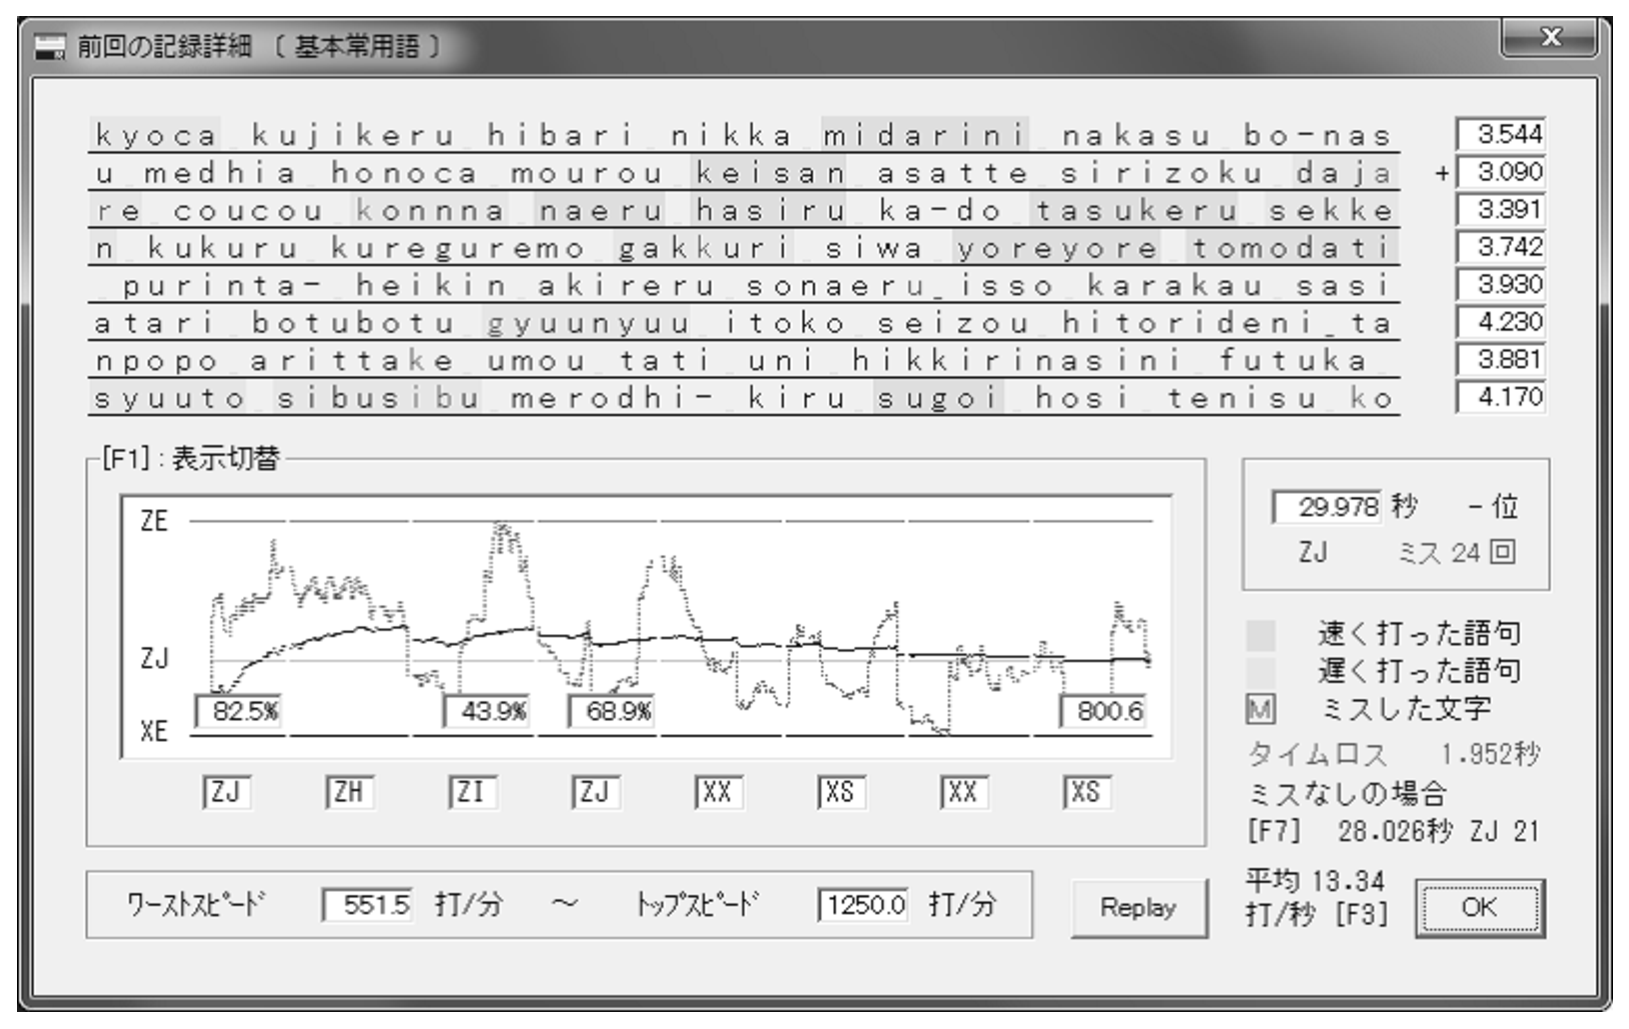
\includegraphics[width=14cm,clip]{res_x_i/tw2.eps}
 \end{center}
 \caption{記録詳細画面}
 \label{x_i:tw_record}
\end{figure*}

\answer{精}{最後まで打ち切ると、こういう画面が出ると思います。「記録詳細」画面ですね。}

\answer{僕}{似たのは出るけど……こんなグラフみたいなのは表示されてないよ。}

\answer{精}{その画面で \key{F1}を何度か押してみてください。押す度に表示が切り替わります。そのうちの一つの表示モードがこのグラフ表示ですね。一番情報量が多いので、玄人はこの表示モードで見ることが多いです。}

\answer{僕}{っていうか超速い記録じゃんこれ! Z とか出てる。}

\answer{精}{私がそれなりに真剣に打つとこんな感じですね。見方はわかります?}

\answer{僕}{わ、わかるよ。……と言いたいとこだけど、よくわからないのもある。}

\answer{精}{打ち切りタイムとか、この打ち切りのレベルとか、ミス回数とかは大丈夫でしょう。}

\answer{僕}{その上に並んでる数字は?}

\answer{精}{「ラップタイム」と呼ばれています。国語Rは400打鍵のタイムを競いますが、それを8のラップに分けて考えることがあります。}

\answer{僕}{各ラップ 50 打鍵……この画面のアルファベットの一行分がラップなんだね。ちょうど 8 行あるから。}

\answer{精}{そういうこと。こうやって分割することで、序盤で速かったけど後半が遅くなった、なんていう大体のプレイ結果を考えやすくしてあるんです。ちなみに各ラップのことを 1 ラップ目、2 ラップ目、なんて呼びますね。}

\answer{僕}{この例だと、3 秒で打っているラップもあれば、4 秒以上かかっているラップもあるね。}

\answer{精}{ラップごとにレベルも表示されていますね。グラフの下にレベルが並んでいるのがそれです。そしてこのグラフでは、もっと細かくスピードの推移を見ることができます。グラフ上の好きな位置にカーソルを合わせると、その地点が上の打鍵内容のどこにあたるのか、またその瞬間の速度はどれくらいだったのか、調べることができるんですよ。}

\answer{僕}{一番スピードが速かった瞬間は…… 3 ラップ目の中盤「萎える」「走る」のあたりか。本当に詳細だ。}

\answer{精}{一番速かったところの速度を「トップスピード」、遅かったところの速度を「ワーストスピード」と呼んでいます。下の方にそれぞれ分速何打のペースか、出てますよね。}

\answer{僕}{一番遅いところでも 551.5……僕の e-typing よりずっと速いってことか。}

\answer{精}{\key{Space}も打鍵にカウントしていますし、ワードごとの小休止なしでずっと続けて打ちますから、e-typing と単純に比較はできないですけど……大体のペースのイメージは湧きますよね。Weather Typing で一瞬だけ高速に打つ練習もしましたから、トップスピード 1250 打/分がどれくらい速いのかも想像がつくんじゃないでしょうか。}

\answer{僕}{「萎える」は\key{U}を中指でっていう最適化を使えば一瞬で打てそうだもんね。}

\answer{精}{e-typing でもやった先読みも駆使して、今打っているワードの次の単語・次の次の単語くらいまでは認識できてますから、組立が間に合えば最適化も使えますね。ワードの種類もそんなに多くない(各モード 2000 程度)ので、ワード慣れもできますし。}

\answer{僕}{今までやってきたことをすべて駆使して挑む……燃えざるを得ないシチュだよ、これは。}

\answer{精}{慣れれば慣れるほど面白いですよ。打つだけでどんどん伸びる時期はそれでいいですけど、伸び悩んできたらこの記録詳細画面で自分の打鍵をよくチェックして、改善点を探したりするといいです。}

\answer{僕}{他にも色々結果を見れる画面があるんだよね?}

\answer{精}{他はいくつもの結果を一覧したり、最高記録を並べたりする画面ですね。個々のプレイの詳細じゃなくて、統計的にどうなのかを見たい時に使います。ショートカットキーが \key{F5}\key{F6}\key{F7} と集中しているので、その辺ポチポチ押してみるといいです。}

\begin{screen}
具体的には、次のような画面です。

\begin{itemize}
 \item トップ15 (\key{F5}):そのモードの自己15位までの記録を一覧。トップスピードやワーストスピードのランキングも。
 \item カナ別成績:各カナごとにかかった平均時間を一覧。
 \item 総合成績(\key{F6}):各モードの最高成績を並べて見られるほか、オンラインランキングで競うことになる総合ポイントが参照できる。
 \item 練習実績(\key{F7}):日々の練習回数、その日の最高タイムなどが参照できる。
\end{itemize}
\end{screen}

\subsection{攻略法?}

単語の間にスペースを挟むのに苦労しながらも何度か打つと、XI が出て、続けて XH が出て……次々に上のランクを出すことができた。

\answer{僕}{XG 出たよ! エーックス! ジー!}

\answer{精}{おめでとうございます。私の予言通りですね。XD くらいまではこのまま行けちゃうと思いますよ。}

\answer{僕}{いつもみたいに、その先へ行くための攻略法も教えてよ。XD なんてすぐ行くから、XA とか ZJ とかのレベルを目指す方法をさ。}

\answer{精}{行き詰まってから言われないとわからないですよー。}

\answer{僕}{もったいぶらないでいいじゃん、もう隠すことなんてないでしょ。}

\answer{精}{それはないですけど……どちらかというと逆で、「これが攻略法だ」って自信満々に教えることができるようなことって、もうそんなにないんですよ。今まで教えて来たようなことをタイプウェルに応用していくだけなんですから。}

\answer{僕}{でも行き詰まったら教えてくれるんでしょ?}

\answer{精}{うーん、つまり、個人差があるのですよ。実際に行き詰まったあなたを見たら、私はきっと「ここが悪い」「ここを改善しよう」ってアドバイスできます。でも今の段階じゃ、あなたがどういうスタイルになって、どこで伸び悩むかなんて、全然わからないわけで。}

\answer{僕}{誰にでも言えるような「攻略法」はない?}

\answer{精}{「スムーズに詰まらず打ちましょう」「速く打てるワードを速く打ちましょう」みたいな中身のないことは言えますよ? でも、実際にどうやって進んでいくかは十人十色。最適化をする・しないの選択だけでもガラッと変わってきますし、もっと細かなタイピングのスタイルによっても話が変わります。あなたがこれから目指すのは、そういう世界です。ゲームとしてソフトを攻略するという部分も少しは残るでしょうけど……それよりも、自分自身を見つめ、分析して、工夫して、練習して、記録を伸ばしていく、その過程・取り組み方が重要になります。}

\answer{僕}{それは、「攻略法」っていうよりは……。}

\answer{精}{「練習法」とでも言ったほうがいいですね。最後はそういう勝負です。知っているだけですごく記録が伸びるテクニックとか裏技……そんなものはこの先、基本的にないです。}

その目はいつになく真剣で、まだ底に残っていた僕の甘えを、見事に射貫いて気化させる。この先の世界こそ、彼女が見ている世界。彼女に追いつき、追い越すために挑まなければいけない世界なのだ。

\answer{僕}{……わかったよ。じゃ、行き詰まったら、アドバイスを頼むね。}

\answer{精}{自分でも考えてくださいよ? 私だって何でもアドバイスできるわけじゃないですから。自分のことは自分が一番よくわかると言いますし、最終的には、すべて自分でわかって、考えることができなきゃダメです。}

その時、僕は一人前になるのだろう。彼女という存在を、越えることができるのだろう。

そしてその時、彼女という存在は、\\
彼女の存在意義は――。

そこまでで、僕は考えることをやめた。左親指でスペースキーを打つ。カウントダウンが始まる。今はまだ、これが僕の見るべき世界だ。

\begin{screen}
攻略法は、いずれ練習論というべきものになっていくよ、と丸投げしてしまいました。入門記事であるこの記事の扱うレベルはここまで、ということです。
これより高度な議論が知りたければ、本物のトップレベルタイパーであるテル氏の執筆された次の記事「タイピング練習論」がそれです。高度な内容を含みますが、ここまでついて来て、実際に競技タイピングの世界に入ることができた方なら、きっと読み解いて、糧にできるはずです。
\end{screen}

\section{文化と天空}
\begin{screen}
冗談じゃねぇ! こんな所! 俺は一人で帰らせてもらうからな!\\
――俺◆gt4Uu5qyB2, 史上初のタイプウェル国語 R 総合 ZG を達成し
\end{screen}

\subsection{環境・目標・交流}
季節は移ろい、制服が衣替えになって久しい。エコという名目でクーラーもつかない学校のパソコン室では、窓という窓が開け放たれ、グラウンドから大会をひかえ力の入っている野球部の快音が響いてくる。

あれから僕は、パソコン部の中に、特にタイピングを専門の活動とするグループを作った。「毎日パソコン入力コンクール」という、僕らが表向き目標にできる大会もあったので、顧問に認めてもらうことは簡単だった。

現在のメンバーは僕を入れて四人。他のメンバーが年上で異性ばかりという環境にもそろそろ慣れて、日々タイピング練習に励んでいる。実力はというと、正直なところ僕以外の皆はまだまだだったが、僕のスピードを目標にしているらしい。成長速度はかなりのもので、ライバルとなれる日も遠くなく思えた。

\begin{screen}
高校生以下の方には「毎日パソコン入力コンクール」への出場を強くおすすめしたいです。\\
\url{http://www.maipaso.net/}

現実社会では大会のようなものが少なく、一般人の評価が得にくい競技タイピングですが、この大会だけは例外です。予選を通過すれば全国大会に出ることができ、さらにそこでも活躍すれば賞品がもらえるほか、立派な表彰も行われます。
甲子園出場並……というとさすがに大げさですが、「全国大会」など響きはすごいので、取り組んで結果を出すことができれば現実生活で大変評価されること間違いなし。昔は一般(専門・大学生・社会人)にも全国大会があったのですが、今では高校生以下しか全国大会への出場権がありませんので、ぜひ中高生のうちに、チャレンジしてみて欲しいと思います。
同年代の人達だけとの勝負なので、この記事で紹介してきたような、究極的で半端じゃなく速い全日本レベルの人でなくても入賞が狙え、現実的でいい目標だと思います。
\end{screen}

僕がこんな行動を起こしたきっかけは、もちろん某ヨウセイサンのささやきがあったからだ。

\answer{精}{ライバルがいると伸びますよ。}

\answer{僕}{少年漫画の基本だねー。適当に GANGAS で探そ。}

\answer{精}{それもいいんですけど、直接会えたり、話せたりする人がいると理想ですね。}

\begin{screen}
とは言うものの、やはりリアルで仲間を作るというのは難しいことも多いでしょう。

最近ですと Twitter 等の SNS でタイパー間の交流が行われているのが目立ちますので、そこに参加するというのを次点でオススメしておきます。「タイプウェル」とか「e-typing」等と検索すればザクザクとタイパーが発見できるでしょう。また本書のあとがきの著者紹介にも、著者勢の Twitter アカウントが載っています。興味がある方は、お気軽にフォロー・リプライしてください。
\end{screen}

……と、思い返していたところに、声をかけられる。

\answer{男}{ねえねえ、今タイプウェルレベル何だっけ?}

\answer{僕}{国語Rは今総合XBになったとこ。今月中には Machine 達成(総合 XA 到達)したいんだよね。}

\answer{男}{成長速ぇーな。全然追いつける気がしないわ。}

\answer{僕}{うーん、けっこう必死だから。……目標設定・自己分析はしてる? 「ひとつ上のレベルを目指すのはもちろんですけど、中期的な目標を立てたりとか、今の自分に足りないのは何かと考えたりとか、そういう意識も大事ですよ」とかなんとか。}

\answer{男}{なるほど……意識からして違うってか。俺はとりあえず Genius 乗せないと始まらないな。ちなみに Machine 乗せた後のことも考えてるわけ?}

\answer{僕}{なんとなくだけど。タイプウェルだけで言っても、英語・オリジナルは全然打ったことないし。全部やるっていうのは大変だけど……やりがいはあると思う。}

\answer{男}{よくやるよなぁ。俺とか国語 R の 4 モードだけで死にそうだ。}

\answer{僕}{やっぱ行き詰まると、他のをやりたくなるじゃん。そういう意味で気分転換にもいいし……色々やると補い合って伸びる部分もあると思うし。何より楽しいよ。新しい種目を苦戦しつつ攻略してくのは。}

\answer{男}{ふーむ、俺は今のとこ、国語 R も行き詰まってはいないからな。}

\answer{僕}{うん、そういう時期はどんどんそれだけやって伸ばしていいでしょ。ただ……タイプウェルばっかりやってるとミスバカになっちゃいがちだから、そういうのは気をつけて。今はまだ、速度重視で伸ばしてもいいと思うけど。}

\answer{男}{ご忠告痛み入るよ。しかし、そんなことまでわかってやってるとか、本当ぱねぇな。}

\answer{僕}{それは……私の場合はちょっと、ずるなんで。}

\answer{男}{ずる?}

\answer{僕}{ううん、何でもない。気にしないで。}

彼に正直に話をしたところで、信じてもらえるはずもないし、証拠も見せられない。今の僕の実力・知識そのものが証拠のようなものだと自分では思うけど……客観的に信用させる証拠たりえないことはわかっていた。

電波女子扱いは、ちょっと困る。オタク趣味だって隠してるんだから。

\subsection{情報発信}

帰宅して、すっかりタイピングソフトで埋め尽くされたデスクトップ画面に向かう。そして意識すれば……。

\answer{精}{おかえりなさいですー。今日もタイピング日和!}

\answer{僕}{やあ。}

彼女が現れる。

\answer{僕}{日和っていうか、毎日やってるじゃん。タイピングに向かない日なんてあるの?}

\answer{精}{ありますよー、寒い日とか。冬になると正直つらいですね。手袋とか靴下とかを手に装着すると暖かくなりますが、打ちにくいですし。}

\answer{僕}{(靴下……?)部屋自体を暖めるしかないのかな。}

\answer{精}{「風呂上がり効果」といって、お湯に手を浸した後だとすごくよく指が動くっていうのが知られています。血行が良くなるからですね。冬でも体ごと暖まりますし……それを利用するのもいいです。}

\answer{僕}{なるほどね……しかし、いつも思うんだけど、どこからそんな知識を仕入れてきてるわけ?}

\answer{精}{もちろん、人づてですよ。先人の知恵と、現役タイパー達の情報交換の中ででしょうか。そうやって今日も明日も明後日も、攻略は積み重なって、続いていくんです。だからあなたも、自分で気づいたこと、思ったことがあったらぜひ積極的に情報発信して欲しいです。}

\answer{僕}{情報発信……ネットのブログとかで?}

\answer{精}{そうです。タイパーをやっている人って、引退後の方も数えれば相当いますけど、現役だけで数えると……そんなにはいないので。貴重なんですよ。あなたみたいなバチバチやってくれる人。}

\answer{僕}{まあ、めちゃくちゃ人が賑わってたら、僕のところに勧誘に来たりしてないよね。}

\answer{精}{立派に成長してくれて私、感激です。}

\answer{僕}{うん。僕こそ最初は何事かと思ったけど……こういう世界があるってわかって良かったと思ってる。}

\answer{精}{泣きそうです。……なので、ついでに気が向いたら、どういう媒体・どういう形式でもいいので、競技タイピングに関したことを形に残してくれると……さらに泣きそうになります。}

\answer{僕}{調子いいんだから……でも、そういえばちょうど今日も部活の人と話したりしてたんだよね。ああいう情報を発信していけばいいのかな。}

\answer{精}{そう、語り尽くされたような情報でもいいんです。同じ事考えてる人がいるなーって誰かが思えるだけで意味がありますしね。それに、自分の記録を積極的に公開していれば、あなたのことをライバル意識してくれる人も増えます。}

\answer{僕}{そうなれば自分のモチベーションにもつながるわけね。いいよ、了解した。}

……と、頭の中で発声する。最近は、彼女を相手にして部屋の中一人で奇声をあげることもなくなった。

彼女に問いを発する頻度が減っていく。何もかも、慣れていく。非現実は現実へと溶けて、\ruby{渾然}{こんぜん}一体となっていく。この頃にはもう、この先に待っていることが何なのか、僕は予感していた。

\subsection{そして高みへ}

まもなくして、タイプウェル国語 R が総合 XA ―― Machine になった。文字通りの「機械」認定。長いようで、振り返ってみるとそうでもなかった道のり。

ここまで行けば調子に乗れる、なんて以前は思っていたけど……実際は全く違った。自分が速くなればなるほど、より速い記録の偉大さがわかってくる。思い上がりや先入観が消えて、純粋に自分の記録・他人の記録を見つめる、競技者としての眼力が養われてくる。

時をおかず、国語 R の Machine よりも難度が高いと言われる e-typing 腕試し 600pt を達成。初速・正確性重視の打ち方も同時に鍛えてきていたおかげなのは、言うまでもない。

速くて正確なタイピング。一体僕は、どこまで来たんだろう? もう、尋ねても良い頃だと思った。しばらくぶりに、彼女に問いかける。

\answer{僕}{ねえ。僕はどこまで来たかな?}

キーボードの上にうっすらと現れた彼女は、じっとこっちを見て、こう答える。

\answer{精}{それは、あなたが一番わかっているはずです。}

\answer{僕}{そうだね。じゃあ次は、何をすればいいかな?}

彼女はきっとこう答える。

\answer{精}{それも、あなたが一番わかっているはずです。}

……その通りなのだ。予感が現実になっていく。それでも、踏み出さなければならない。僕を導いてくれた、彼女を越えていくために。

\answer{僕}{じゃあ次が最後だよ。}

\answer{精}{はい}

\answer{僕}{僕は、君が望んだ僕になれたかな?}

\answer{精}{……もちろんです。}

満足そうに、でも少しだけ名残惜しそうに笑って、彼女はその姿を消した。

いなくなったわけではない。今もここに。しばらくの間、僕は刻印のはがれかかったキーボードから、目を離せないでいた。

こうして、あるべき形に、僕たちは戻った。

\section*{終章}
\begin{screen}
一生を棒に降りし男ここに眠る。彼は無価値に生きたり。\\
――高村光太郎、墓碑銘
\end{screen}

ふと我に返る。

集中し過ぎたのだろうか。記録更新ペースでの最終ラップ――その最中に一瞬、意識が飛んだようだった。

にもかかわらず……画面には「新記録樹立!」の文字が映し出されている。

打ち始める前に、高校時代のことを思い出していたからだろうか。何だか、追体験をしたような感覚がある。

――そこで僕は、未熟な誰かにタイピングを教えるのだ。

閃きが落ちてくる。可能性に過ぎないと思う一方で、僕はその解釈を受け入れたい気持ちで満たされた。

\answer{僕}{「『私は、どこまで行くんでしょう?』」}

――楽しいと思える限り、どこまでも。

